% chapters/03_diseño_experimental.tex
\chapter{Experimentación y resultados}
\label{chap:diseno_experimental}

Este capítulo traslada el marco teórico anterior al diseño experimental del trabajo. El objetivo es evaluar el uso de procesos gaussianos como modelos sustitutos probabilísticos para aproximar una relación entre configuraciones de entrada y una respuesta de interés, especialmente en escenarios donde las evaluaciones son limitadas o costosas.

La experimentación se organiza en dos escenarios. En primer lugar, se utilizan funciones benchmark sintéticas, donde la función objetivo es conocida y puede evaluarse en nuevos puntos. Este escenario permite estudiar el ciclo completo de optimización basada en modelos sustitutos: diseño inicial, ajuste del GP, selección secuencial de puntos mediante un criterio de \emph{infill} y actualización del conjunto observado. En segundo lugar, se plantea un caso real basado en datos experimentales de dietas para insectos. En este caso, las observaciones proceden de ensayos ya realizados y se encuentran agrupadas por dieta, por lo que el objetivo principal no es ejecutar nuevas evaluaciones físicas, sino validar si el modelo generaliza a dietas no vistas.

Por tanto, ambos escenarios comparten el mismo marco general de modelado sustituto, pero no el mismo protocolo experimental: los benchmarks permiten analizar el proceso secuencial de búsqueda en un entorno controlado, mientras que el caso real evalúa la viabilidad del enfoque antes de plantear una fase prospectiva de recomendación de nuevas configuraciones.

\section{Marco común de modelado sustituto}
\label{subsec:marco_comun_modelado_sustituto}

En ambos escenarios se parte de un conjunto finito de observaciones
\[
    \mathcal{D}_n = \{(\bm{x}_i, y_i)\}_{i=1}^{n},
\]
donde \(\bm{x}_i \in \mathcal{X}\) representa una configuración de entrada e \(y_i\) la respuesta observada. A partir de estos datos se entrena un modelo sustituto cuyo objetivo es aproximar la relación entre entradas y salidas, proporcionando predicciones en configuraciones no observadas y, en el caso de los procesos gaussianos, una estimación de incertidumbre.

\subsection{Datos, modelos y preprocesamiento}
\label{subsubsec:representacion_datos}

Las entradas se organizan en una matriz de diseño \(X \in \mathbb{R}^{n \times d}\), donde \(n\) es el número de observaciones y \(d\) la dimensión del espacio de entrada. Las respuestas se recogen en un vector \(\bm{y} \in \mathbb{R}^{n}\). En los benchmarks, cada observación corresponde a una evaluación controlada de una función sintética. En el caso real, cada observación corresponde a una medición experimental asociada a una dieta, por lo que las particiones de entrenamiento y evaluación deben respetar dicha agrupación para evitar fuga de información entre réplicas de una misma dieta.

El diseño experimental considera dos modelos. El modelo Dummy se utiliza como línea base mínima para comprobar si el GP aporta capacidad predictiva frente a una predicción trivial. El proceso gaussiano constituye el modelo sustituto principal y se implementa mediante la clase \texttt{GPSurrogateRegressor}, construida a partir de un \texttt{Pipeline} que integra el escalado de variables y el ajuste de un \texttt{GaussianProcessRegressor}.

El preprocesamiento se realiza siempre dentro del \texttt{Pipeline}, de modo que el escalado se ajusta únicamente con los datos de entrenamiento de cada partición o iteración experimental. Esto evita utilizar información del conjunto de evaluación durante el ajuste. En el caso real, las transformaciones adicionales necesarias para representar las dietas se describen en el apartado específico correspondiente.

\subsection{Predicción probabilística e incertidumbre}
\label{subsubsec:prediccion_incertidumbre}

Para una nueva configuración \(\bm{x}\), el GP devuelve una media predictiva \(\mu(\bm{x})\) y una desviación típica \(\sigma(\bm{x})\). La media se utiliza como predicción puntual y la desviación típica como medida de incertidumbre. En los benchmarks, esta incertidumbre se usa de forma activa dentro de Expected Improvement (EI) para seleccionar nuevas evaluaciones. En el caso real, se emplea como indicador de fiabilidad de las predicciones, sin ejecutar todavía una fase física de \emph{infill}.

\subsection{Métricas comunes}
\label{subsubsec:metricas_comunes}

La evaluación reutiliza las métricas predictivas y probabilísticas introducidas en el estado del arte, junto con una métrica específica para analizar el éxito del proceso de optimización en los benchmarks. Las primeras evalúan la calidad del GP como modelo predictivo; la última mide si el proceso de \emph{infill} permite encontrar mejores valores de la función objetivo.

\begin{table}[htbp]
    \centering
    \caption{Familias de métricas utilizadas en la evaluación experimental.}
    \label{tab:metricas_experimentales}
    \begin{tabular}{p{3.4cm} p{4.5cm} p{5.7cm}}
        \toprule
        \textbf{Familia} & \textbf{Métricas} & \textbf{Interpretación} \\
        \midrule
        Predictivas 
        & MAE, RMSE, \(R^2\) 
        & Evalúan el error de la predicción puntual. \\

        Probabilísticas 
        & NLPD, cobertura del 95\%
        & Evalúan la calidad de la incertidumbre predictiva. \\

        Optimización 
        & \textit{clean best found}, reducción relativa del \textit{gap}
        & Evalúan si el proceso de \emph{infill} mejora el mínimo encontrado. \\
        \bottomrule
    \end{tabular}
\end{table}
\FloatBarrier

En los benchmarks, la métrica principal de optimización se define como
\[
    I_t = \frac{g_0 - g_t}{g_0},
\]
donde \(g_0\) es la distancia inicial al óptimo y \(g_t\) la distancia al óptimo tras \(t\) iteraciones de \emph{infill}. Valores cercanos a cero indican poca mejora respecto al diseño inicial, mientras que valores cercanos a uno indican una reducción casi completa de la distancia inicial al óptimo. En Borehole, al no disponer de un valor óptimo definido en la implementación, se emplea la reducción relativa del mejor valor limpio encontrado respecto al diseño inicial.

En consecuencia, los benchmarks se analizan desde una doble perspectiva: la evolución del mínimo encontrado y la calidad predictiva del GP durante el proceso secuencial. En el caso real, donde no se ejecutan nuevas evaluaciones físicas, el análisis se centra en la generalización a dietas no vistas mediante agregaciones por partición de validación.

\section{Experimento 1: benchmarks sintéticos}
\label{subsec:experimento_benchmarks}

El primer experimento se desarrolla sobre funciones benchmark sintéticas, donde la función objetivo puede evaluarse en nuevos puntos del dominio. Esto permite analizar el ciclo completo de optimización basada en modelos sustitutos: partir de un diseño inicial, ajustar un GP, seleccionar nuevas evaluaciones mediante Expected Improvement (EI) y actualizar secuencialmente el conjunto observado. El objetivo no es solo medir el error final del modelo, sino estudiar cómo evolucionan el mejor valor encontrado, la capacidad predictiva y la incertidumbre a medida que se incorporan nuevas observaciones.

\subsection{Benchmarks seleccionados}
\label{subsubsec:benchmarks_seleccionados}

Se consideran cuatro benchmarks con una progresión razonable de dificultad, desde problemas de baja dimensión e interpretación visual hasta funciones de mayor dimensión que deben analizarse principalmente mediante métricas. Los dominios de búsqueda se definen en la implementación y se utilizan de forma común para el muestreo inicial, el conjunto de test y la optimización del criterio de adquisición.

\begin{table}[htbp]
    \centering
    \small
    \caption{Benchmarks seleccionados para el experimento sintético.}
    \label{tab:benchmarks_seleccionados}
    \renewcommand{\arraystretch}{1.15}
    \setlength{\tabcolsep}{5pt}
    \begin{tabularx}{\textwidth}{@{}p{2.4cm} c p{3.8cm} X@{}}
        \toprule
        \textbf{Benchmark} & \textbf{Dim.} & \textbf{Dominio} & \textbf{Papel en el experimento} \\
        \midrule

        Forrester 
        & 1 
        & \(x \in [0,1]\)
        & Caso unidimensional para visualizar el ajuste del GP, la incertidumbre y el comportamiento de EI. \\

        Branin 
        & 2 
        & \(x_1 \in [-5,10]\), \(x_2 \in [0,15]\)
        & Función bidimensional multimodal, útil para analizar la selección de puntos en un dominio representable. \\

        Hartmann6 
        & 6 
        & \(x_i \in [0,1]\), \(i=1,\dots,6\)
        & Benchmark de mayor dimensión y multimodalidad, evaluado principalmente mediante métricas. \\

        Borehole 
        & 8 
        & Dominio heterogéneo de ocho variables
        & Problema de inspiración ingenieril para estudiar el comportamiento del método en dimensión superior. \\

        \bottomrule
    \end{tabularx}
\end{table}
\FloatBarrier

\subsection{Diseño inicial, presupuesto y configuraciones GP}
\label{subsec:diseno_inicial_presupuesto}

Para cada benchmark se genera un diseño inicial dentro del dominio de búsqueda, que representa la información disponible antes de iniciar el proceso secuencial de \emph{infill}. Se comparan dos estrategias de muestreo inicial, Sobol y muestreo aleatorio uniforme, y tres tamaños iniciales:
\[
    n_{\text{train}} \in \{1,\; 1 \times d,\; 4 \times d\},
\]
donde \(d\) es la dimensión del benchmark. El caso \(n_{\text{train}}=1\) permite observar el comportamiento del sistema desde una situación extrema con una única observación inicial, mientras que \(1 \times d\) y \(4 \times d\) representan diseños escalados con la dimensión del problema.

A partir del diseño inicial, el proceso de \emph{infill} añade \(5 \times d\) nuevos puntos, sujeto a un máximo de 50 observaciones durante la trayectoria. También se consideran tres condiciones de ruido: evaluación sin ruido y ruido gaussiano con niveles \(0.5\) y \(1.0\).

\begin{table}[htbp]
    \centering
    \caption{Configuración general del experimento de benchmarks.}
    \label{tab:configuracion_benchmarks}
    \begin{tabular}{p{4.1cm} p{11.1cm}}
        \toprule
        \textbf{Elemento} & \textbf{Configuración} \\
        \midrule
        Benchmarks 
        & Forrester, Branin, Hartmann6 y Borehole. \\

        Muestreo inicial 
        & Sobol y aleatorio uniforme. \\

        Tamaño inicial 
        & \(n_{\text{train}} = 1\), \(1 \times d\) y \(4 \times d\). \\

        Presupuesto de \emph{infill} 
        & \(5 \times d\) puntos añadidos al diseño inicial, con un máximo de 50 observaciones durante el proceso. \\

        Ruido 
        & Sin ruido y ruido gaussiano con niveles \(0.5\) y \(1.0\). \\

        Modelos GP 
        & Kernels Matérn \(3/2\), Matérn \(5/2\), RBF y lineal; en dimensión mayor que uno se evalúan versiones isotrópicas y con ARD. \\

        Conjunto de test 
        & Conjunto independiente generado dentro del dominio de cada benchmark. \\

        Semillas 
        & Se utilizan semillas fijas para garantizar la reproducibilidad del experimento. La configuración detallada se recoge en el Anexo~\ref{app:semillas_benchmarks}. \\
        \bottomrule
    \end{tabular}
\end{table}
\FloatBarrier

El dominio detallado de Borehole, el flujo completo del proceso de \emph{infill} y la configuración específica de semillas se incluyen como material complementario en el Anexo~\ref{app:benchmarks_complementario}. En particular, el dominio de Borehole se recoge en la Tabla~\ref{tab:app_dominio_borehole}, el esquema del proceso secuencial en la Figura~\ref{fig:app_flujo_infill} y las semillas empleadas en la Tabla~\ref{tab:app_semillas_benchmarks}.


En cada iteración, el GP se ajusta con el conjunto de observaciones disponible \(\mathcal{D}_n\). A continuación, se calcula EI sobre el dominio de búsqueda y se selecciona el siguiente punto como
\[
    \bm{x}_{\mathrm{next}}
    =
    \operatorname*{arg\,max}_{\bm{x}\in\mathcal{X}} EI(\bm{x}).
\]
Aunque la función objetivo se plantea como un problema de minimización, EI se maximiza porque representa la mejora esperada respecto al mejor valor observado hasta el momento. En la implementación, la maximización de EI se aproxima mediante Differential Evolution; los detalles del procedimiento de optimización de la función de adquisición se recogen en el Anexo~\ref{app:flujo_infill}.


\paragraph{Criterios de lectura del experimento.}
\label{subsec:criterios_analisis_benchmarks}
Antes de presentar los resultados, conviene fijar la lectura del experimento. El análisis se centra en tres bloques: la evolución del mejor valor encontrado durante el proceso de \emph{infill}, la evolución de la capacidad predictiva del GP, incluyendo el diagnóstico de incertidumbre, y el efecto de factores como el tamaño inicial, el ruido, la dimensionalidad, el kernel y el uso de ARD.

\subsection{Resultados del experimento benchmark}
\label{subsec:resultados_benchmarks}

Los resultados se organizan en tres niveles. Primero se analiza si el proceso de \emph{infill} basado en EI mejora el mejor valor encontrado de la función objetivo. Después se estudia si las nuevas observaciones también mejoran la capacidad predictiva del GP. Finalmente, se resumen los factores experimentales que más condicionan el rendimiento observado.

\subsubsection{Evolución del mínimo encontrado durante el proceso de infill}
\label{subsubsec:resultados_incumbent_benchmarks}

La métrica principal desde el punto de vista de la optimización es la mejora relativa del \emph{incumbent}, definida en la Sección~\ref{subsubsec:metricas_comunes}. En este análisis, \emph{step}=0 representa el mejor punto disponible en el diseño inicial, antes de añadir nuevas evaluaciones. A partir de ahí, cada iteración incorpora el punto seleccionado por EI y actualiza el mejor valor encontrado.

La Tabla~\ref{tab:resumen_incumbent_benchmarks} resume el mejor modelo de cada benchmark según la mejora final del \emph{incumbent}. También se incluye la mejora acumulada, que permite distinguir si la mejora aparece pronto durante la trayectoria o si se concentra al final del presupuesto de \emph{infill}.

La mejora acumulada se calcula a partir del área bajo la trayectoria normalizada de mejora del \emph{incumbent}. Por tanto, no solo mide el resultado final, sino también la rapidez con la que aparece la mejora. Un ratio cercano a uno indica que la mayor parte de la mejora se obtiene pronto, mientras que un ratio menor sugiere una mejora más tardía.

\begin{table}[h]
\centering
\small
\caption{Resumen del mejor modelo de optimización por benchmark. La mejora final mide el resultado al terminar el proceso de \emph{infill}; la mejora acumulada resume la evolución durante la trayectoria.}
\label{tab:resumen_incumbent_benchmarks}
\begin{tabularx}{\textwidth}{@{}p{1.8cm}p{3.1cm}ccccX@{}}
\toprule
Benchmark & Mejor modelo & Mejora final & Mejora acum. & Ratio & \(n_{\text{train}}\) & Lectura \\
\midrule
Borehole & \(GP\_Linear\) & \(0.720\) & \(0.694\) & \(0.963\) & \(1\) & Mejora temprana y fuerte. \\
Branin & \(GP\_Matern52\_ARD\) & \(0.898\) & \(0.596\) & \(0.663\) & \(1\) & Mejora final muy alta. \\
Forrester & \(GP\_Matern52\) & \(0.737\) & \(0.390\) & \(0.530\) & \(4\) & Mejora fuerte, pero más tardía. \\
Hartmann6 & \(GP\_RBF\) & \(0.434\) & \(0.304\) & \(0.701\) & \(24\) & Mejora moderada en mayor dimensión. \\
\bottomrule
\end{tabularx}
\end{table}
\FloatBarrier

Los resultados muestran que EI consigue mejoras positivas en los cuatro benchmarks, aunque con distinta intensidad. Branin presenta la mejora final más clara, con una reducción media del \emph{gap} cercana a \(0.90\). Forrester y Borehole también muestran mejoras elevadas, mientras que Hartmann6 resulta el escenario más exigente: la mejora existe, pero es más moderada y requiere un diseño inicial más informativo, coherente con su mayor dimensionalidad.

\begin{figure}[h]
    \centering
    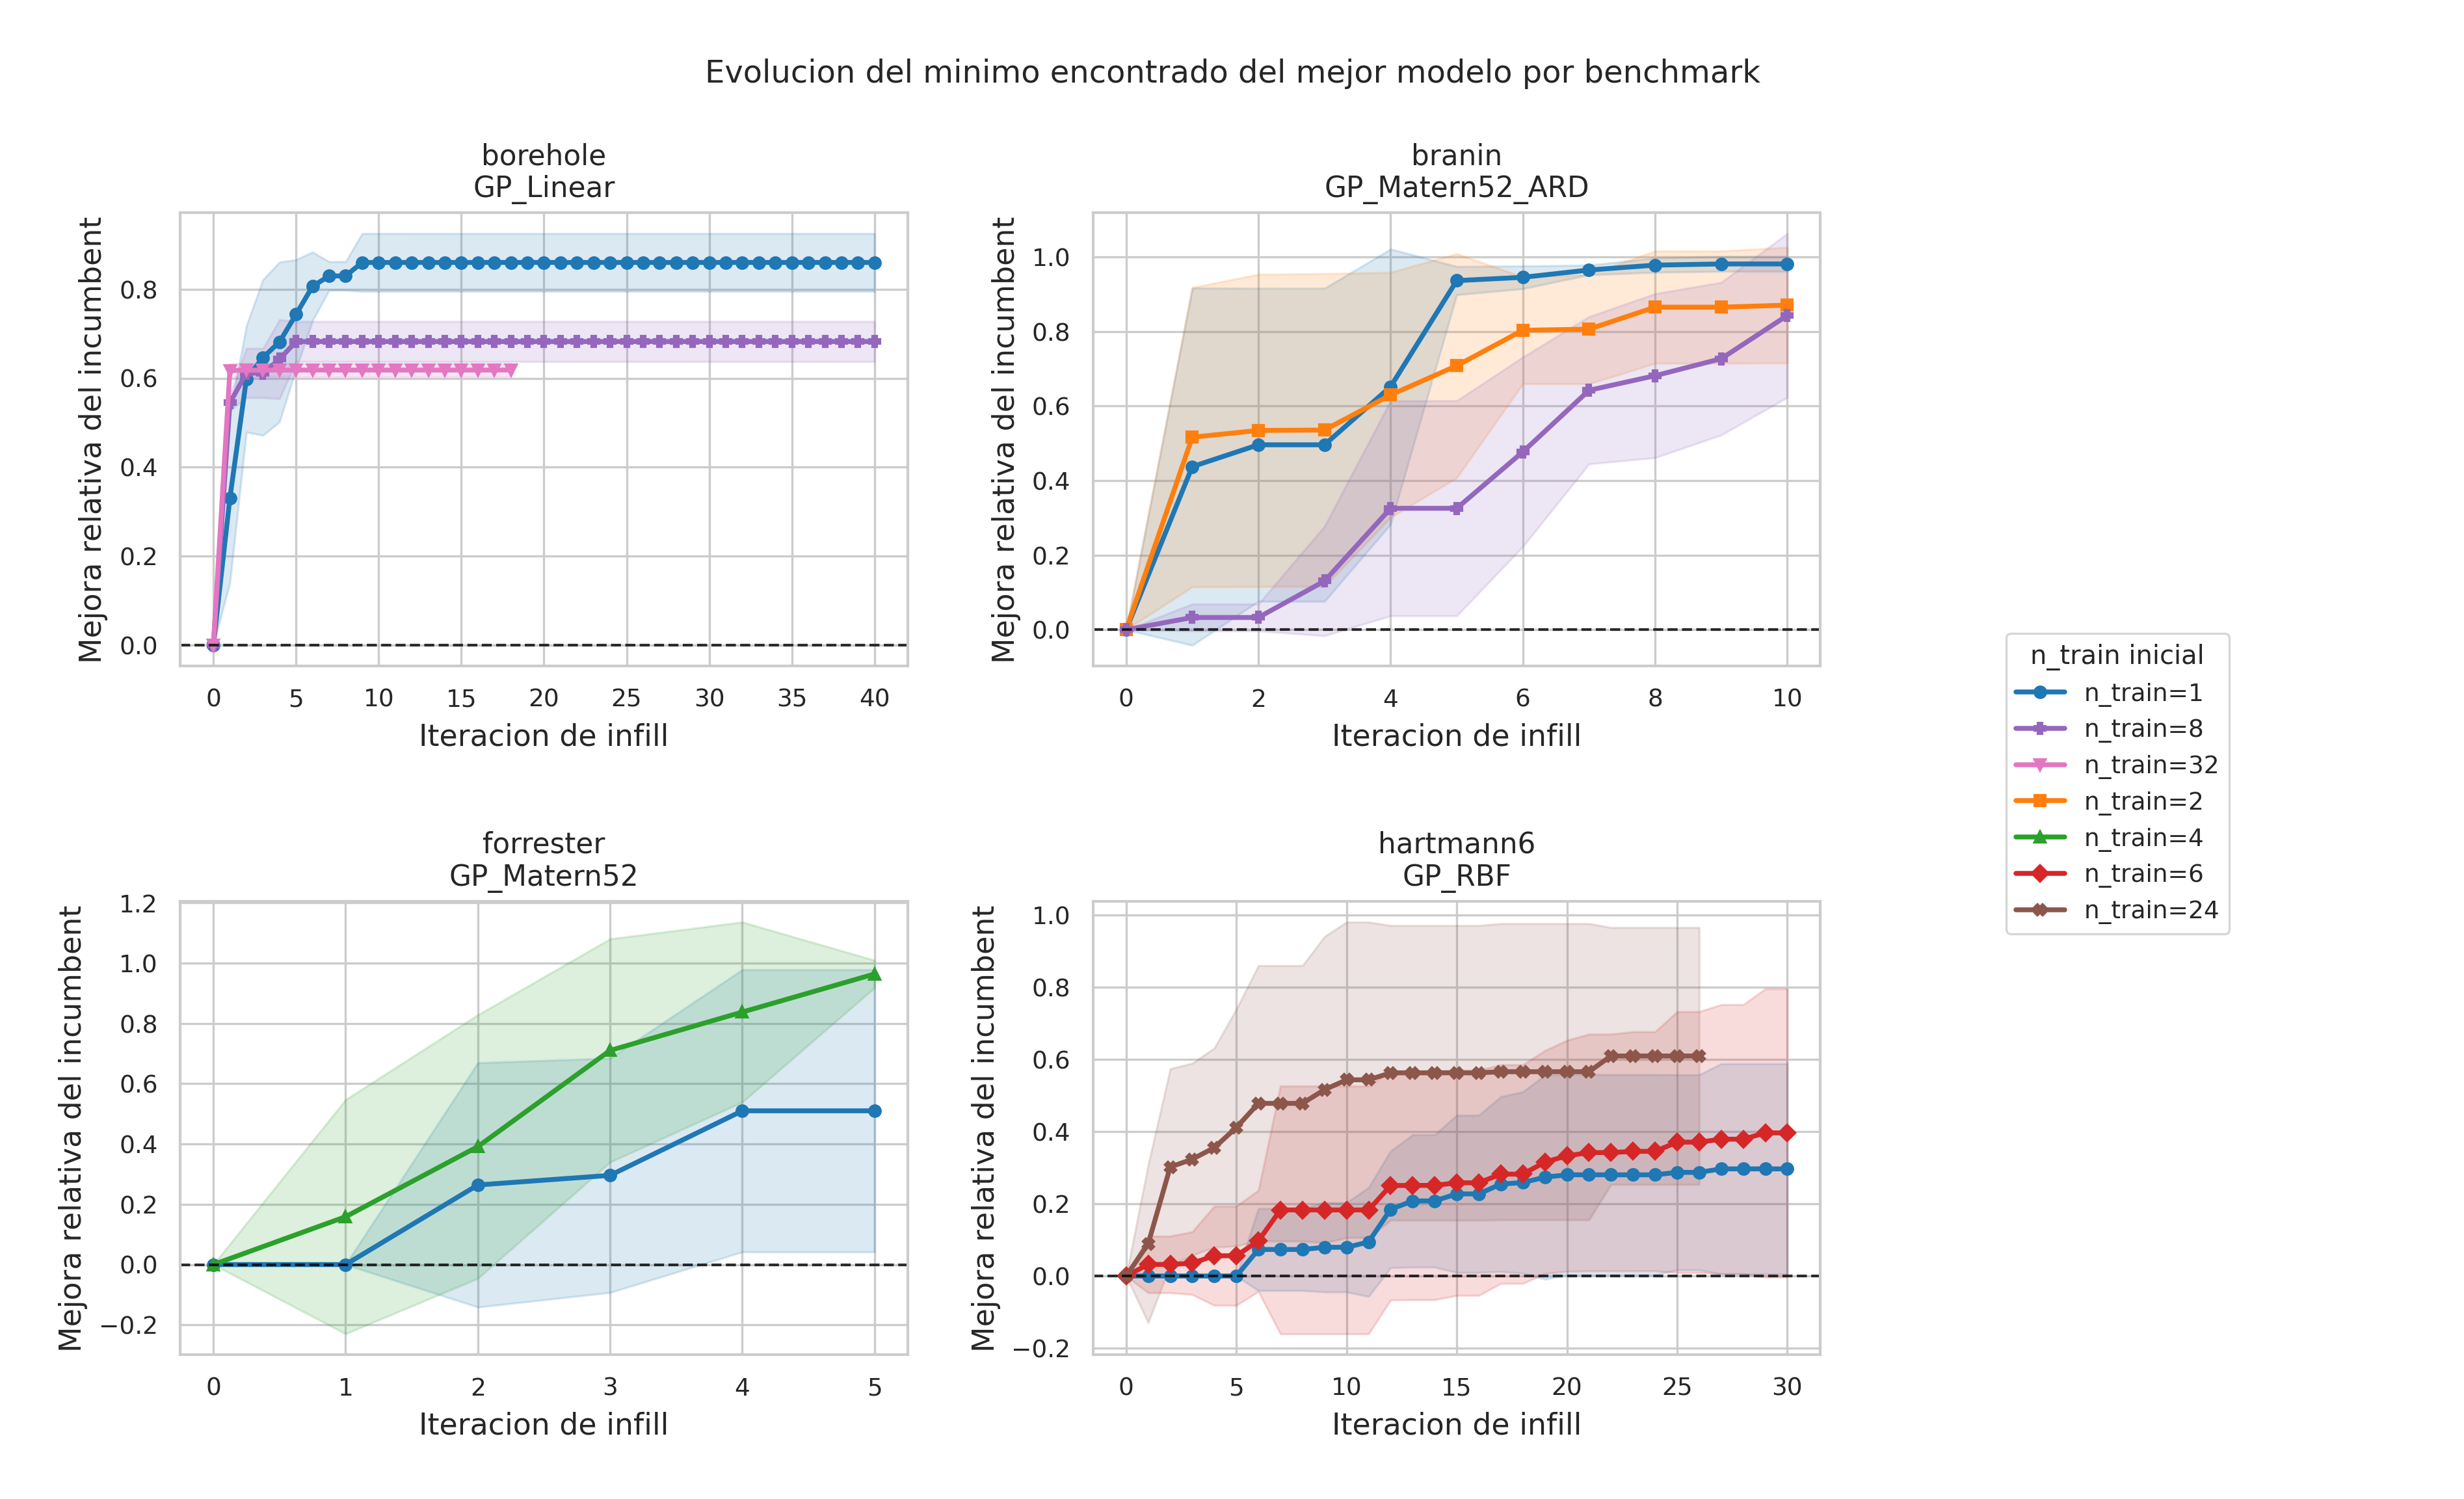
\includegraphics[width=1\textwidth]{assets/evolution_incumbent_best_model_by_benchmark.png}
    \caption{Evolución de la mejora relativa del mínimo encontrado para el mejor modelo de cada benchmark. El valor \emph{step}=0 corresponde al mejor punto del diseño inicial, antes de añadir puntos mediante EI. Las curvas muestran la media y las bandas sombreadas la desviación típica.}
    \label{fig:evolution_incumbent_best_model}
\end{figure}
\FloatBarrier


En Borehole, la mejora final y la mejora acumulada son muy próximas, lo que indica que el proceso encuentra regiones favorables desde fases tempranas. En Branin, la mejora final es muy alta, aunque parte del progreso aparece a lo largo de la trayectoria. Forrester presenta una mejora final fuerte, pero menos inmediata. En Hartmann6, el progreso es más gradual, lo que confirma que el presupuesto disponible resulta más restrictivo en problemas de mayor dimensión.

La Figura~\ref{fig:evolution_incumbent_best_model} confirma esta lectura temporal. En Borehole y Branin, gran parte de la mejora aparece durante las primeras iteraciones y después las curvas tienden a estabilizarse. En Forrester, la trayectoria depende más del diseño inicial y la mejora aparece de forma menos inmediata. En Hartmann6, el avance es más progresivo, lo que refuerza la importancia de disponer de más información inicial en problemas de mayor dimensión. Como material complementario, la Figura~\ref{fig:app_final_relative_incumbent_improvement} muestra la mejora relativa final del \emph{incumbent} agregada por benchmark.

En conjunto, el análisis del \emph{incumbent} confirma que EI cumple su función principal dentro del ciclo de optimización: seleccionar nuevas evaluaciones que mejoran el mejor valor encontrado respecto al diseño inicial. Sin embargo, la magnitud, estabilidad y rapidez de la mejora dependen del benchmark, del kernel y de la cantidad de información inicial disponible.

\subsubsection{Evolución de la capacidad predictiva del GP}
\label{subsubsec:resultados_mae_benchmarks}

Además del éxito en optimización, se analiza si el proceso de \emph{infill} mejora la capacidad predictiva del GP. Para ello se utiliza principalmente el MAE relativo respecto al estado inicial. Esta lectura debe separarse de la mejora del \emph{incumbent}: una configuración puede predecir mejor en promedio sobre el conjunto de test sin ser necesariamente la más útil para encontrar mínimos.

La Tabla~\ref{tab:resumen_predictivo_benchmarks} resume el mejor modelo predictivo de cada benchmark y su comparación frente a Dummy. Dummy no participa en el proceso de \emph{infill}, pero sirve como referencia para comprobar si el GP aporta valor frente a una predicción trivial.

\begin{table}[h]
\centering
\small
\caption{Resumen de la mejora predictiva del GP y comparación frente a Dummy.}
\label{tab:resumen_predictivo_benchmarks}
\begin{tabular}{llccc}
\toprule
Benchmark & Mejor modelo MAE & Mejora MAE & Ganancia vs Dummy & \% mejor que Dummy \\
\midrule
Borehole & \(GP\_RBF\_ARD\) & \(0.574\) & \(0.847\) & \(100.0\%\) \\
Branin & \(GP\_RBF\) & \(0.175\) & \(0.280\) & \(72.2\%\) \\
Forrester & \(GP\_RBF\) & \(0.281\) & \(0.291\) & \(66.7\%\) \\
Hartmann6 & \(GP\_Linear\) & \(0.466\) & \(0.306\) & \(94.4\%\) \\
\bottomrule
\end{tabular}
\end{table}
\FloatBarrier

El GP aporta valor predictivo frente a Dummy en todos los benchmarks, aunque con distinta intensidad. La mejora es especialmente clara en Borehole y Hartmann6, mientras que en Branin y Forrester es más moderada e irregular. Sin embargo, los mejores modelos predictivos no coinciden siempre con los mejores modelos de optimización. Por ejemplo, en Hartmann6 el mejor modelo según MAE es \(GP\_Linear\), pero el mejor modelo para mejorar el \emph{incumbent} es \(GP\_RBF\). De forma similar, \(GP\_RBF\) destaca en MAE para Branin y Forrester, mientras que los mejores modelos de optimización son \(GP\_Matern52\_ARD\) y \(GP\_Matern52\), respectivamente.

Las métricas probabilísticas se interpretan como diagnóstico complementario. En conjunto, el proceso de \emph{infill} tiende a reducir simultáneamente el MAE y el NLPD respecto al estado inicial, aunque la calibración de la incertidumbre no es uniforme entre benchmarks. En Borehole y Branin se observa subcobertura en todos los modelos, lo que sugiere intervalos predictivos demasiado estrechos. En Forrester y Hartmann6 la cobertura se aproxima más al valor nominal en algunas configuraciones. Por tanto, la incertidumbre del GP resulta útil para guiar EI y diagnosticar la fiabilidad de las predicciones, pero no debe confundirse con una garantía directa de éxito en optimización.

Estos resultados confirman que la precisión global, la calibración probabilística y la utilidad para guiar la búsqueda del óptimo son aspectos relacionados, pero no equivalentes. Por ello, en este experimento se analizan por separado la mejora del mínimo encontrado y la evolución de la capacidad predictiva del modelo. Las figuras complementarias del Anexo~\ref{app:benchmarks_complementario} muestran con más detalle la evolución relativa del MAE y el diagnóstico conjunto entre MAE, NLPD y cobertura predictiva; véanse las Figuras~\ref{fig:app_evolution_relative_mae_best_model} y~\ref{fig:app_mae_vs_probabilistic_diagnostics}.

\subsubsection{Influencia de las condiciones experimentales}
\label{subsubsec:influencia_condiciones_benchmarks}

Finalmente, se resume el efecto agregado de las condiciones experimentales evaluadas. Dado el elevado número de combinaciones, el objetivo no es describir cada configuración de forma aislada, sino identificar qué factores parecen condicionar más el rendimiento del proceso GP + EI.

La Tabla~\ref{tab:jerarquia_factores_benchmark} muestra que el factor más determinante es el propio benchmark. La dificultad de la función, asociada a la dimensionalidad y a la estructura del paisaje objetivo, condiciona más el rendimiento que decisiones aisladas como el sampler o el uso de ARD. El tamaño del diseño inicial también es relevante: en problemas sencillos pueden bastar pocas observaciones para orientar la búsqueda, mientras que en problemas más complejos un diseño inicial mayor ayuda a estabilizar el proceso.

Respecto al kernel, no se observa una configuración universalmente superior. Los kernels Matérn y RBF destacan en distintos benchmarks, mientras que el kernel lineal puede comportarse razonablemente como predictor global en algunos casos, pero no necesariamente como guía de optimización. Por su parte, ARD, el sampler y el ruido muestran efectos más irregulares y dependientes del contexto experimental. 

En conjunto, el rendimiento del proceso GP + EI depende principalmente de tres elementos: la dificultad del benchmark, la cantidad de información inicial disponible y la adecuación del kernel a la estructura de la función. Los demás factores influyen, pero no presentan una ventaja sistemática en el análisis agregado. El análisis gráfico de los efectos emparejados de estas condiciones se recoge como material complementario en la Figura~\ref{fig:app_factor_effects_paired}.

\begin{table}[h]
\centering
\small
\caption{Jerarquía de factores experimentales observada en el experimento benchmark.}
\label{tab:jerarquia_factores_benchmark}
\begin{tabularx}{\textwidth}{@{}p{0.9cm}p{2.8cm}XX@{}}
\toprule
\textbf{Orden} & \textbf{Factor} & \textbf{Evidencia} & \textbf{Interpretación} \\
\midrule

1 
& Benchmark/dimensionalidad 
& Mejor \emph{incumbent} entre \(0.434\) y \(0.898\) según benchmark. 
& Factor dominante; condiciona la dificultad del problema y el margen de mejora. \\

2 
& \(n_{\text{train}}\) inicial 
& Rango de mejora: Forrester \(0.457\), Branin \(0.365\). 
& Muy relevante, aunque debe interpretarse junto al valor final y no solo mediante mejora relativa. \\

3 
& Kernel 
& Borehole: \(GP\_Linear\); Branin: \texttt{GP\_Matern52\_ARD}; Forrester: \texttt{GP\_Matern52}; Hartmann6: \texttt{GP\_RBF}. 
& Importa, pero depende del benchmark; no hay un ganador universal. \\

4 
& ARD 
& \(\Delta=0.002\), \(46\,\%\) favorable, \(n=108\). 
& No muestra una ventaja universal en \emph{incumbent}; puede ser más útil en MAE. \\

5 
& Sampler 
& \(\Delta=0.035\), \(38\,\%\) favorable, \(n=186\). 
& Efecto secundario e irregular frente a benchmark, diseño inicial y kernel. \\

6 
& Ruido 
& \(\Delta=0.110\) para \(\sigma=0.5\), \(\Delta=0.125\) para \(\sigma=1.0\). 
& Afecta a la estabilidad del proceso, aunque su efecto agregado depende del contexto. \\

\bottomrule
\end{tabularx}
\end{table}
\FloatBarrier


\section{Experimento 2: caso real con dietas para insectos}
\label{subsec:experimento_caso_real}

El segundo experimento traslada el marco de modelos sustitutos a un caso real basado en datos experimentales de cría de insectos. En este contexto, el interés se centra en la fase larvaria, ya que es la fase utilizada posteriormente como fuente de alimentación. El problema experimental consiste en estudiar cómo distintas formulaciones de dieta afectan al crecimiento de las larvas y a su composición final.

El diseño experimental parte de una dieta control, compuesta únicamente por salvado de trigo. Esta dieta representa la referencia habitual de cría y permite comparar el efecto de introducir dietas no convencionales. Las dietas no convencionales mantienen el salvado de trigo como base, pero sustituyen una parte por un subproducto alimentario con valor nutricional. En el estudio principal se consideran tres subproductos: hoja de olivo, cascarilla de quinoa y orujo de oliva.

Desde el punto de vista del modelado, el objetivo no es únicamente ajustar un modelo a una tabla de datos, sino evaluar si un GP puede capturar relaciones útiles entre la composición de la dieta y la respuesta observada en las larvas. Estas relaciones son relevantes porque los ensayos físicos son limitados y cada nueva formulación requiere una validación experimental. Por tanto, el modelo sustituto se plantea como una herramienta previa para estimar respuestas y cuantificar incertidumbre antes de una posible fase prospectiva de selección de nuevas dietas.

Las respuestas de interés combinan parámetros productivos y variables de composición. En el plano productivo, una variable relevante es \texttt{FCR}, que mide la relación entre la cantidad de alimento consumido y la ganancia de peso obtenida. Valores menores de \texttt{FCR} indican una conversión más eficiente del alimento en biomasa. En el plano composicional, se consideran variables como \texttt{PROTEINA (\%)} y \texttt{QUITINA (\%)}. En las primeras pruebas tambien se consideró \texttt{TPC} que recoge la concentración de compuestos fenólicos totales en las larvas tras la cría y se utiliza como indicador adicional asociado al efecto de la dieta pero no se analizarán sus resultados.

En consecuencia, el caso real persigue dos objetivos metodológicos. En primer lugar, comprobar si el GP es capaz de generalizar a dietas no vistas a partir de variables de composición, inclusión y tipo de subproducto. En segundo lugar, analizar si la incertidumbre predictiva puede servir como señal de fiabilidad del modelo. A diferencia del experimento con \emph{benchmarks} sintéticos, aquí no se ejecuta un ciclo secuencial de \emph{infill}, ya que las observaciones proceden de ensayos experimentales ya realizados.

\subsection{Alcance del caso real y selección de \textit{Hermetia}}
\label{subsec:alcance_hermetia_caso_real}

El archivo experimental original contiene información para dos especies: \textit{Hermetia illucens} y \textit{Tenebrio molitor}. Además, recoge varios bloques de información: composición nutricional y TPC de las dietas, parámetros productivos de la cría y composición nutricional y TPC de las larvas obtenidas. Sin embargo, los resultados modelados en este experimento se limitan al dataset \texttt{productivity\_hermetia\_lote.csv}.

Esta decisión no implica que los datos de \textit{Tenebrio} sean inválidos. La razón es de alcance experimental y homogeneidad del caso modelado. El bloque de \textit{Hermetia} utilizado en el pipeline contiene 33 observaciones, organizadas en 11 dietas con 3 réplicas por dieta, todas pertenecientes al mismo bloque de estudio. Además, las covariables necesarias para los dos modos de entrada están completas y los objetivos presentan una disponibilidad suficientemente homogénea: \texttt{FCR} cuenta con 31 valores válidos y \texttt{QUITINA (\%)} y \texttt{PROTEINA (\%)} cuentan con 33 valores.

En cambio, aunque \textit{Tenebrio} también se genera como dataset procesado, mezcla varios bloques experimentales y tipos adicionales de dieta, como los asociados a posos de café y orujillo. Estos datos incorporan diferencias de tratamiento, especialmente en la forma de suministrar agua en algunos controles, y presentan una disponibilidad distinta de objetivos. Por ello, \textit{Tenebrio} se reserva como posible segundo caso o subanálisis posterior, pero no se mezcla con \textit{Hermetia} en los resultados actuales.

\subsection{Diseño experimental y dietas consideradas}
\label{subsec:diseno_dietas_caso_real}

El dataset modelado contiene una dieta control y varias dietas no convencionales. La dieta \texttt{Control} corresponde al salvado de trigo sin inclusión de subproductos y actúa como referencia experimental. Las dietas no convencionales se nombran combinando el subproducto utilizado y su porcentaje de inclusión. Así, por ejemplo, \texttt{Hoja15}, \texttt{Hoja30} y \texttt{Hoja50} indican dietas con 15 \%, 30 \% y 50 \% de hoja de olivo, respectivamente. La misma lógica se aplica a las dietas con orujo de oliva y cascarilla de quinoa.

Cada dieta se administra a tres lotes de larvas, por lo que el análisis se realiza a nivel de réplica experimental. Esta decisión conserva la variabilidad entre lotes y evita reducir prematuramente el dataset a medias por dieta. La columna \texttt{diet\_name} identifica la dieta asociada a cada réplica y se utiliza posteriormente como variable de agrupación en la validación.

\begin{table}[htbp]
    \centering
    \small
    \caption{Resumen del dataset utilizado en el caso real.}
    \label{tab:dataset_caso_real}
    \renewcommand{\arraystretch}{1.12}
    \begin{tabular}{ll}
        \toprule
        \textbf{Elemento} & \textbf{Descripción} \\
        \midrule
        Dataset modelado & \texttt{productivity\_hermetia\_lote.csv} \\
        Especie & \textit{Hermetia illucens} \\
        Observaciones & 33 réplicas experimentales \\
        Dietas & 11 dietas \\
        Réplicas por dieta & 3 \\
        Dieta de referencia & \texttt{Control}, basada en salvado de trigo \\
        Subproductos principales & Hoja de olivo, orujo de oliva y cascarilla de quinoa \\
        Variable de grupo & \texttt{diet\_name} \\
        Objetivos & \texttt{FCR}, \texttt{QUITINA (\%)}, \texttt{PROTEINA (\%)} \\
        Nivel de trabajo & Réplica experimental \\
        \bottomrule
    \end{tabular}
\end{table}

La representación de entrada combina variables de formulación y composición de la dieta. Se consideran dos conjuntos de variables. El modo reducido, \texttt{REDUCED\_FEATURES}, incluye \texttt{inclusion\_pct}, \texttt{Proteína (\%)\_media}, \texttt{Fibra (\%)\_media}, \texttt{Grasa (\%)\_media} y \texttt{TPC\_dieta\_media}. El modo completo, \texttt{FULL\_FEATURES}, añade \texttt{Cenizas (\%)\_media}, \texttt{Carbohidratos (\%)\_media} y tres ratios nutricionales derivados. En ambos casos se incorporan variables binarias asociadas al tipo de subproducto mediante la codificación de \texttt{byproduct\_type}.

De este modo, el modelo no utiliza únicamente el nombre de la dieta como identificador, sino una descripción estructurada de cada formulación. Esta representación permite estudiar si las variables disponibles contienen información suficiente para anticipar la respuesta de dietas completas no vistas durante el entrenamiento.

\subsection{Limpieza y preprocesamiento}
\label{subsec:preprocesamiento_caso_real}

El dataset utilizado en el caso real se obtiene a partir del archivo experimental original mediante un proceso de limpieza, combinación y transformación de tablas. El objetivo de esta etapa es pasar de varias hojas de Excel, con información distribuida por tipo de análisis, a una tabla única a nivel de réplica experimental. En esa tabla, cada fila debe contener tanto la respuesta observada como las variables necesarias para describir la dieta evaluada.

El proceso seguido puede resumirse en los siguientes pasos.

\begin{description}
    \item[\textbf{Paso 1. Limpieza de las hojas originales.}]
    En primer lugar, se normalizan las hojas correspondientes a composición de dieta, parámetros productivos, composición larvaria y TPC. Durante esta etapa se corrigen nombres de columnas duplicados, se homogeneizan tratamientos y se estructuran las columnas de medias y desviaciones. También se normalizan los nombres de las variables que se utilizarán posteriormente en el modelado.

    \item[\textbf{Paso 2. Enumeración de réplicas.}]
    Para poder unir correctamente las distintas fuentes de información, se asigna un identificador de réplica dentro de cada dieta. Este paso es necesario porque los parámetros productivos y la composición de larvas se registran a nivel de lote o réplica de cría. De este modo, cada observación final puede asociarse a una dieta concreta y a una réplica experimental concreta.

    \item[\textbf{Paso 3. Construcción del dataset de productividad.}]
    Una vez limpias las tablas originales, se construye el dataset de productividad de \textit{Hermetia}. Para ello, se combinan los parámetros productivos con la composición larvaria usando como claves la dieta, el tratamiento, la réplica y la especie. Después, se añade la composición nutricional de la dieta y la información de TPC. El resultado es una tabla a nivel de réplica que integra información productiva, composición de larva y descripción de la dieta.

    \item[\textbf{Paso 4. Extracción de metadatos de dieta.}]
    A partir del nombre textual de cada dieta se generan variables estructuradas, como \texttt{diet\_name}, \texttt{byproduct\_type} e \texttt{inclusion\_pct}. Esta transformación permite que el modelo no dependa únicamente del nombre de la dieta, sino de variables interpretables: tipo de subproducto, porcentaje de inclusión y composición nutricional. Además, se calculan ratios nutricionales derivados que se emplean en el modo completo de variables.

    \item[\textbf{Paso 5. Selección del objetivo y filtrado de valores ausentes.}]
    El modelado se realiza de forma independiente para cada variable objetivo. Para cada objetivo se eliminan únicamente las filas cuyo valor de respuesta está ausente. Esta decisión evita descartar observaciones válidas para el resto de objetivos. Así, \texttt{FCR} se evalúa con 31 observaciones válidas, mientras que \texttt{QUITINA (\%)} y \texttt{PROTEINA (\%)} se evalúan con las 33 observaciones disponibles.

    \item[\textbf{Paso 6. Construcción de \(X\), \(\bm{y}\) y grupos.}]
    Para cada objetivo se construye la matriz de entrada \(X\), el vector de respuesta \(\bm{y}\) y el vector de grupos. El vector \(\bm{y}\) contiene los valores observados del objetivo seleccionado. El vector de grupos se construye a partir de \texttt{diet\_name}, de forma que todas las réplicas de una misma dieta compartan el mismo identificador de grupo. Esta agrupación será la base del protocolo LODO descrito en la Sección~\ref{subsec:lodo_caso_real}.

    \item[\textbf{Paso 7. Codificación de variables categóricas.}]
    Las variables de entrada se forman combinando las variables numéricas seleccionadas con una codificación binaria del tipo de subproducto. En concreto, \texttt{byproduct\_type} se transforma en variables indicadoras y se concatena con las variables numéricas del modo reducido o completo. Todas las columnas resultantes se convierten a formato numérico antes del ajuste del modelo.

    \item[\textbf{Paso 8. Escalado dentro del \texttt{Pipeline}.}]
    El escalado de variables se realiza dentro del \texttt{Pipeline} de cada modelo. Por tanto, los parámetros de normalización se estiman únicamente con los datos de entrenamiento de cada partición y se aplican después sobre la dieta retenida en test.
\end{description}

En el CSV final utilizado, las variables de entrada seleccionadas no presentan valores ausentes. Por tanto, la imputación por mediana incluida en la construcción de \(X\) no modifica los datos en esta versión del experimento. En conjunto, este preprocesamiento transforma los datos experimentales originales en una estructura supervisada y agrupada por dieta. Esta organización permite evaluar el modelo en una situación más exigente que una partición aleatoria por filas: predecir la respuesta de dietas completas no observadas durante el entrenamiento.


\subsection{Protocolo de evaluación Leave-One-Diet-Out}
\label{subsec:lodo_caso_real}

La evaluación del caso real se realiza mediante un protocolo \emph{Leave-One-Diet-Out} (LODO), motivado por la estructura agrupada del dataset. Las observaciones no son muestras independientes sin relación entre sí, sino réplicas experimentales asociadas a una misma dieta. Por tanto, una partición aleatoria por filas podría situar réplicas de una misma dieta simultáneamente en entrenamiento y test, generando una estimación demasiado optimista de la capacidad predictiva del modelo. A continuación, se presenta el protocolo LODO en la Figura~\ref{fig:nested_lodo}.

\begin{figure}[h]
    \centering
    \resizebox{0.98\textwidth}{!}{%
    \begin{tikzpicture}[
        >=Latex,
        font=\small,
        panel/.style={
            draw,
            rounded corners=8pt,
            thick,
            inner sep=0pt
        },
        box/.style={
            draw,
            rounded corners=4pt,
            thick,
            align=center,
            inner sep=5pt
        },
        greenbox/.style={box, fill=green!18},
        bluebox/.style={box, fill=blue!16},
        orangebox/.style={box, fill=orange!18},
        pinkbox/.style={box, fill=pink!20},
        smallbox/.style={
            draw,
            rounded corners=3pt,
            thick,
            minimum width=0.78cm,
            minimum height=0.34cm
        },
        dietbox/.style={
            draw,
            rounded corners=2pt,
            thick,
            fill=yellow!20,
            minimum width=0.82cm,
            minimum height=0.95cm,
            align=center,
            font=\scriptsize
        },
        testbox/.style={
            draw,
            rounded corners=2pt,
            thick,
            fill=blue!18,
            minimum width=0.82cm,
            minimum height=0.95cm,
            align=center,
            font=\scriptsize
        },
        arr/.style={->, thick}
    ]

    % =====================================================
    % MARCO GENERAL
    % =====================================================
    \node[panel, minimum width=16.0cm, minimum height=15.6cm] (frame) at (0,0) {};

    % Título general
    \node[anchor=north west, font=\bfseries] at (-7.35,7.20)
    {Nested LODO: validación anidada \emph{Leave-One-Diet-Out}};

    % =====================================================
    % OUTER LODO
    % =====================================================
    \node[anchor=north west, font=\Large\bfseries] at (-7.05,6.55)
    {Outer LODO};

    \node[
        anchor=north west,
        font=\footnotesize,
        text=green!45!black,
        align=left,
        text width=5.9cm
    ] at (-7.05,5.98)
    {Una dieta completa se deja fuera para\\[-1mm]
     medir el rendimiento final};

    \node[
        pinkbox,
        minimum width=3.25cm,
        minimum height=0.90cm,
        anchor=north east
    ] at (6.50,6.62) {
        \(P\) dietas \(\rightarrow\) \(P\) folds\\[-1mm]
        \scriptsize una partición por dieta
    };

    % Texto central sin líneas laterales
    \node[font=\Large] (fold) at (0,5.12) {Para cada fold};

    % Etiquetas izquierda / derecha
    \node[anchor=north, align=center] (trainlbl) at (-4.20,4.55) {
        Dietas restantes\\[-1mm]
        \scriptsize \(X_{\text{train}},\, y_{\text{train}},\, g_{\text{train}}\)
    };

    \node[anchor=north, align=center] (testlbl) at (4.20,4.55) {
        Dieta retenida\\[-1mm]
        \scriptsize \(X_{\text{test}},\, y_{\text{test}},\, g_{\text{test}}\)
    };

    \draw[arr] (-2.05,4.88) -- (trainlbl.north);
    \draw[arr] ( 2.05,4.88) -- (testlbl.north);

\begin{scope}[yshift=-0.45cm]
    % =====================================================
    % INNER LODO
    % =====================================================
    % Bajado para que no pise train/test
    \node[panel, minimum width=14.30cm, minimum height=5.00cm] (inner) at (0,1.15) {};

    \node[anchor=north west, font=\Large\bfseries] at (-6.75,3.45)
    {Inner LODO};

    \node[
        anchor=north west,
        font=\footnotesize,
        text=green!45!black,
        align=left,
        text width=8.5cm
    ] at (-6.75,2.95)
    {Validación interna para seleccionar hiperparámetros};

    % Grid title separado del subtítulo y de los cuadrados
    \node[
    anchor=north west,
    text=blue!70!black,
    font=\bfseries
    ] at (-6.65,2.45)
    {Grid de parámetros};
    
    \foreach \x in {-5.95,-5.05,-4.15,-3.25,-2.35,-1.45,-0.55} {
        \node[smallbox] at (\x,1.62) {};
    }
    
    \node[
        greenbox,
        minimum width=1.30cm,
        minimum height=0.76cm,
        font=\scriptsize
    ] (best) at (1.00,1.62) {
        mejores\\[-1mm]params
    };

    % Fold interno
    \node[
        anchor=north west,
        align=left,
        text width=2.4cm
    ] at (-6.65,0.92)
    {Para cada\\[-1mm]fold interno};

    % Línea entrenamiento
    \draw[thick] (-4.10,0.72) -- (-0.85,0.72);
    \node[font=\scriptsize, fill=white, inner sep=1pt] at (-2.48,0.96)
    {Entrenamiento};

    % Dietas con separación uniforme
    \node[dietbox] at (-3.80,0.00) {Dieta\\[-1mm]1};
    \node[dietbox] at (-2.90,0.00) {Dieta\\[-1mm]2};
    \node[dietbox] at (-2.00,0.00) {Dieta\\[-1mm]3};
    \node[dietbox] at (-1.10,0.00) {Dieta\\[-1mm]4};
    \node[testbox] at (-0.05,0.00) {Test};

    % Flecha curva reposicionada para no pisar "fold"
    \draw[arr]
    (-6.00,0.15)
    .. controls (-6.10,-0.55) and (-5.05,-0.55)
    .. (-4.45,-0.05);

    \node[
        anchor=west,
        align=left,
        text=green!45!black
    ] (generalizan) at (1.85,0.00) {
        parámetros que\\[-1mm]
        mejor generalizan
    };

    \draw[arr] (best.south east) -- (generalizan.north west);
    \end{scope}
    % =====================================================
    % EVALUACIÓN EXTERNA
    % =====================================================
    \node[panel, minimum width=14.30cm, minimum height=2.45cm] (eval) at (0,-3.20) {};

    \node[anchor=north west, font=\large\bfseries] at (-6.65,-2.15)
    {Evaluación externa};

    \node[
        greenbox,
        minimum width=3.85cm,
        minimum height=0.85cm
    ] (fit) at (-4.05,-3.40) {
        Reentrenar modelo\\[-1mm]
        \scriptsize con los mejores parámetros
    };

    \node[
        bluebox,
        minimum width=3.60cm,
        minimum height=0.76cm
    ] (pred) at (0.00,-3.40) {
        Predecir sobre \(X_{\text{test}}\)
    };

    \node[
        orangebox,
        minimum width=4.60cm,
        minimum height=0.85cm
    ] (metric) at (4.50,-3.40) {
        Calcular métricas externas\\[-1mm]
        \scriptsize con \(y_{\text{test}}\)
    };

    \draw[arr] (fit.east) -- (pred.west);
    \draw[arr] (pred.east) -- (metric.west);

    % =====================================================
    % RESULTADOS AGREGADOS
    % =====================================================
    \begin{scope}[yshift=0.45cm]
    \node[font=\Large\bfseries] at (0,-5.68)
    {Resultados agregados};

    % Cuadros con separación uniforme
    \node[box, minimum width=2.55cm, minimum height=0.95cm] at (-4.70,-6.58) {
    MAE\\[-1mm]
    \scriptsize media y desviación
    };
    
    \node[box, minimum width=2.55cm, minimum height=0.95cm] at (-1.7,-6.58) {
        RMSE\\[-1mm]
        \scriptsize media y desviación
    };
    
    \node[box, minimum width=2.95cm, minimum height=0.95cm] at (1.40,-6.58) {
        Cobertura 95\,\%\\[-1mm]
        \scriptsize media y desviación
    };
    
    \node[box, minimum width=3.55cm, minimum height=0.95cm] at (4.93,-6.58) {
        Mejores parámetros\\[-1mm]
        \scriptsize por fold externo
    };
    \end{scope}
    \end{tikzpicture}%
    }
     \caption{Esquema del protocolo de validación anidada \emph{Leave-One-Diet-Out}. En cada fold externo se deja fuera una dieta completa para evaluar el rendimiento final. La selección de hiperparámetros se realiza mediante una validación interna sobre las dietas restantes.}
    \label{fig:nested_lodo}
\end{figure}
\FloatBarrier

Sea \(\mathcal{G}=\{g_1,\dots,g_K\}\) el conjunto de dietas disponibles. En el fold externo \(k\), el conjunto de test queda formado por todas las observaciones pertenecientes a la dieta \(g_k\):
\[
    \mathcal{D}_{\text{test}}^{(k)}
    =
    \{(\bm{x}_i,y_i): g_i = g_k\}.
\]
El conjunto de entrenamiento contiene el resto de dietas:
\[
    \mathcal{D}_{\text{train}}^{(k)}
    =
    \{(\bm{x}_i,y_i): g_i \in \mathcal{G}\setminus\{g_k\}\}.
\]
De este modo, todas las réplicas de la dieta retenida quedan excluidas del ajuste. En el dataset de \textit{Hermetia}, al disponer de 11 dietas, el protocolo genera 11 folds externos.

La selección de hiperparámetros se realiza de forma anidada. Para cada fold externo, la dieta retenida se reserva exclusivamente para la evaluación final. Sobre las dietas restantes se ejecuta una validación interna, también basada en grupos, y se selecciona la configuración con menor MAE. A continuación, el modelo se reentrena con todas las observaciones del entrenamiento externo y se evalúa sobre la dieta retenida.

Este diseño evalúa una tarea más exigente que interpolar entre réplicas de dietas ya observadas. El modelo debe predecir la respuesta de una dieta completa que no ha participado ni en el ajuste final ni en la selección de hiperparámetros. Por ello, los resultados obtenidos con LODO se interpretan como una estimación de la capacidad de generalización a dietas no vistas dentro del espacio experimental disponible.

\subsection{Modelos, ajuste y métricas}
\label{subsec:modelos_metricas_caso_real}

En esta etapa se comparan una línea base simple y varias configuraciones de GP. Todos los modelos se evalúan bajo el protocolo LODO anidado descrito en la Sección~\ref{subsec:lodo_caso_real}, de forma independiente para cada objetivo y para cada modo de representación de entrada: \texttt{REDUCED\_FEATURES} y \texttt{FULL\_FEATURES}.

\begin{table}[htbp]
    \centering
    \small
    \caption{Modelos considerados en el caso real.}
    \label{tab:modelos_caso_real}
    \renewcommand{\arraystretch}{1.12}
    \begin{tabular}{p{0.28\textwidth}p{0.62\textwidth}}
        \toprule
        \textbf{Modelo} & \textbf{Descripción} \\
        \midrule
        \texttt{Dummy} &
        Línea base constante, basada en media o mediana del conjunto de entrenamiento. Sirve como referencia mínima. \\

        \texttt{GP\_Linear} &
        GP con kernel lineal y término de ruido blanco. Representa una hipótesis de relación aproximadamente lineal entre variables de dieta y respuesta. \\

        \texttt{GP\_RBF\_NoARD} &
        GP con kernel RBF escalar y ruido blanco. Introduce una hipótesis suave y no lineal con una escala común para las variables de entrada. \\

        \texttt{GP\_Matern32\_NoARD} &
        GP con kernel Matérn \(\nu=1.5\) y ruido blanco. Permite funciones menos suaves que RBF. \\

        \texttt{GP\_Matern52\_NoARD} &
        GP con kernel Matérn \(\nu=2.5\) y ruido blanco. Supone una respuesta más suave que Matérn \(3/2\), pero menos restrictiva que RBF. \\

        \texttt{GP\_Compuesto\_NoARD} &
        GP con kernel aditivo lineal + Matérn \(5/2\) + ruido blanco. Combina una componente lineal con una componente no lineal suave. \\

        Variante ARD selectiva &
        Versión con escalas por variable aplicada solo al mejor kernel previo de cada combinación de objetivo y modo de variables. \\
        \bottomrule
    \end{tabular}
\end{table}

El ajuste se organiza en tres niveles:

\begin{description}
    \item[\textbf{Selección interna.}]
    En cada fold externo, los parámetros se seleccionan mediante un LODO interno aplicado únicamente sobre las dietas de entrenamiento. La métrica de selección es el MAE, por lo que se elige la configuración con menor error absoluto medio en validación interna.

    \item[\textbf{Evaluación externa.}]
    Una vez seleccionados los parámetros, el modelo se reentrena con todas las dietas del entrenamiento externo y se evalúa sobre la dieta retenida. Las métricas finales proceden de esta evaluación externa, no del entrenamiento. En los modelos GP se obtiene tanto la media predictiva como la desviación típica. Esta segunda magnitud permite calcular métricas asociadas a incertidumbre. 
\end{description}

La lectura de métricas se apoya en las definiciones introducidas en la Sección~\ref{subsubsec:metricas_comunes}. En este caso, el MAE se utiliza como métrica principal para seleccionar hiperparámetros y comparar modelos. RMSE y \(R^2\) se emplean como diagnósticos secundarios: RMSE ayuda a detectar errores grandes y \(R^2\) aporta una lectura global del ajuste, aunque debe interpretarse con cautela por el reducido número de réplicas por dieta. Para los GP, NLPD y cobertura del intervalo predictivo al 95 \% se utilizan como diagnósticos de incertidumbre, no como criterios de selección.

Las métricas externas se agregan de dos formas. La agregación macro calcula la media simple de los folds externos, de modo que cada dieta retenida pesa lo mismo. Esta es la lectura principal del caso real, porque el objetivo es evaluar generalización por dieta y no dar más peso a dietas con más réplicas válidas. La agregación micro pondera por el número de muestras de cada fold y se utiliza únicamente como comprobación secundaria. En los resultados se prioriza, por tanto, el MAE macro sobre los folds externos.

\subsection{Resultados del caso real}
\label{subsec:resultados_caso_real}

Los resultados del caso real se analizan con una lectura distinta a la del experimento de benchmarks. En este escenario solo se dispone de un conjunto limitado de ensayos experimentales ya realizados. Por tanto, el interés principal no es medir únicamente el error medio del modelo, sino comprobar si el GP aprende relaciones que puedan transferirse a dietas completas no observadas durante el entrenamiento.

\subsubsection{Generalización estructural frente a memorización}
\label{subsubsec:generalizacion_lodo_caso_real}

La primera cuestión es si el modelo sustituto es capaz de extraer una señal general a partir de las variables de formulación y composición, o si su rendimiento depende únicamente de reconocer dietas ya presentes en el entrenamiento. Para responder a esta pregunta se utiliza el protocolo LODO descrito en la Sección~\ref{subsec:lodo_caso_real}. En cada fold externo se deja fuera una dieta completa, de modo que ninguna de sus réplicas participa ni en el ajuste del modelo ni en la selección de hiperparámetros. Así, la evaluación reproduce una situación más exigente que una partición aleatoria por filas: el modelo debe predecir la respuesta de una formulación no vista.

La Figura~\ref{fig:lodo_generalization_vs_dummy} resume el rendimiento relativo frente al modelo Dummy. El eje vertical representa el MAE normalizado respecto al Dummy, por lo que valores inferiores a \(1\) indican mejora frente a la predicción trivial. Bajo esta lectura, el GP compuesto mejora al Dummy en los tres objetivos activos: la reducción relativa del error es del \(15.8\,\%\) en FCR, del \(15.4\,\%\) en quitina y del \(36.6\,\%\) en proteína. Este resultado indica que el modelo no se limita a reproducir una media global, sino que aprovecha información contenida en las variables de entrada para anticipar, al menos parcialmente, la respuesta de dietas no vistas.

\begin{figure}[htbp]
    \centering
    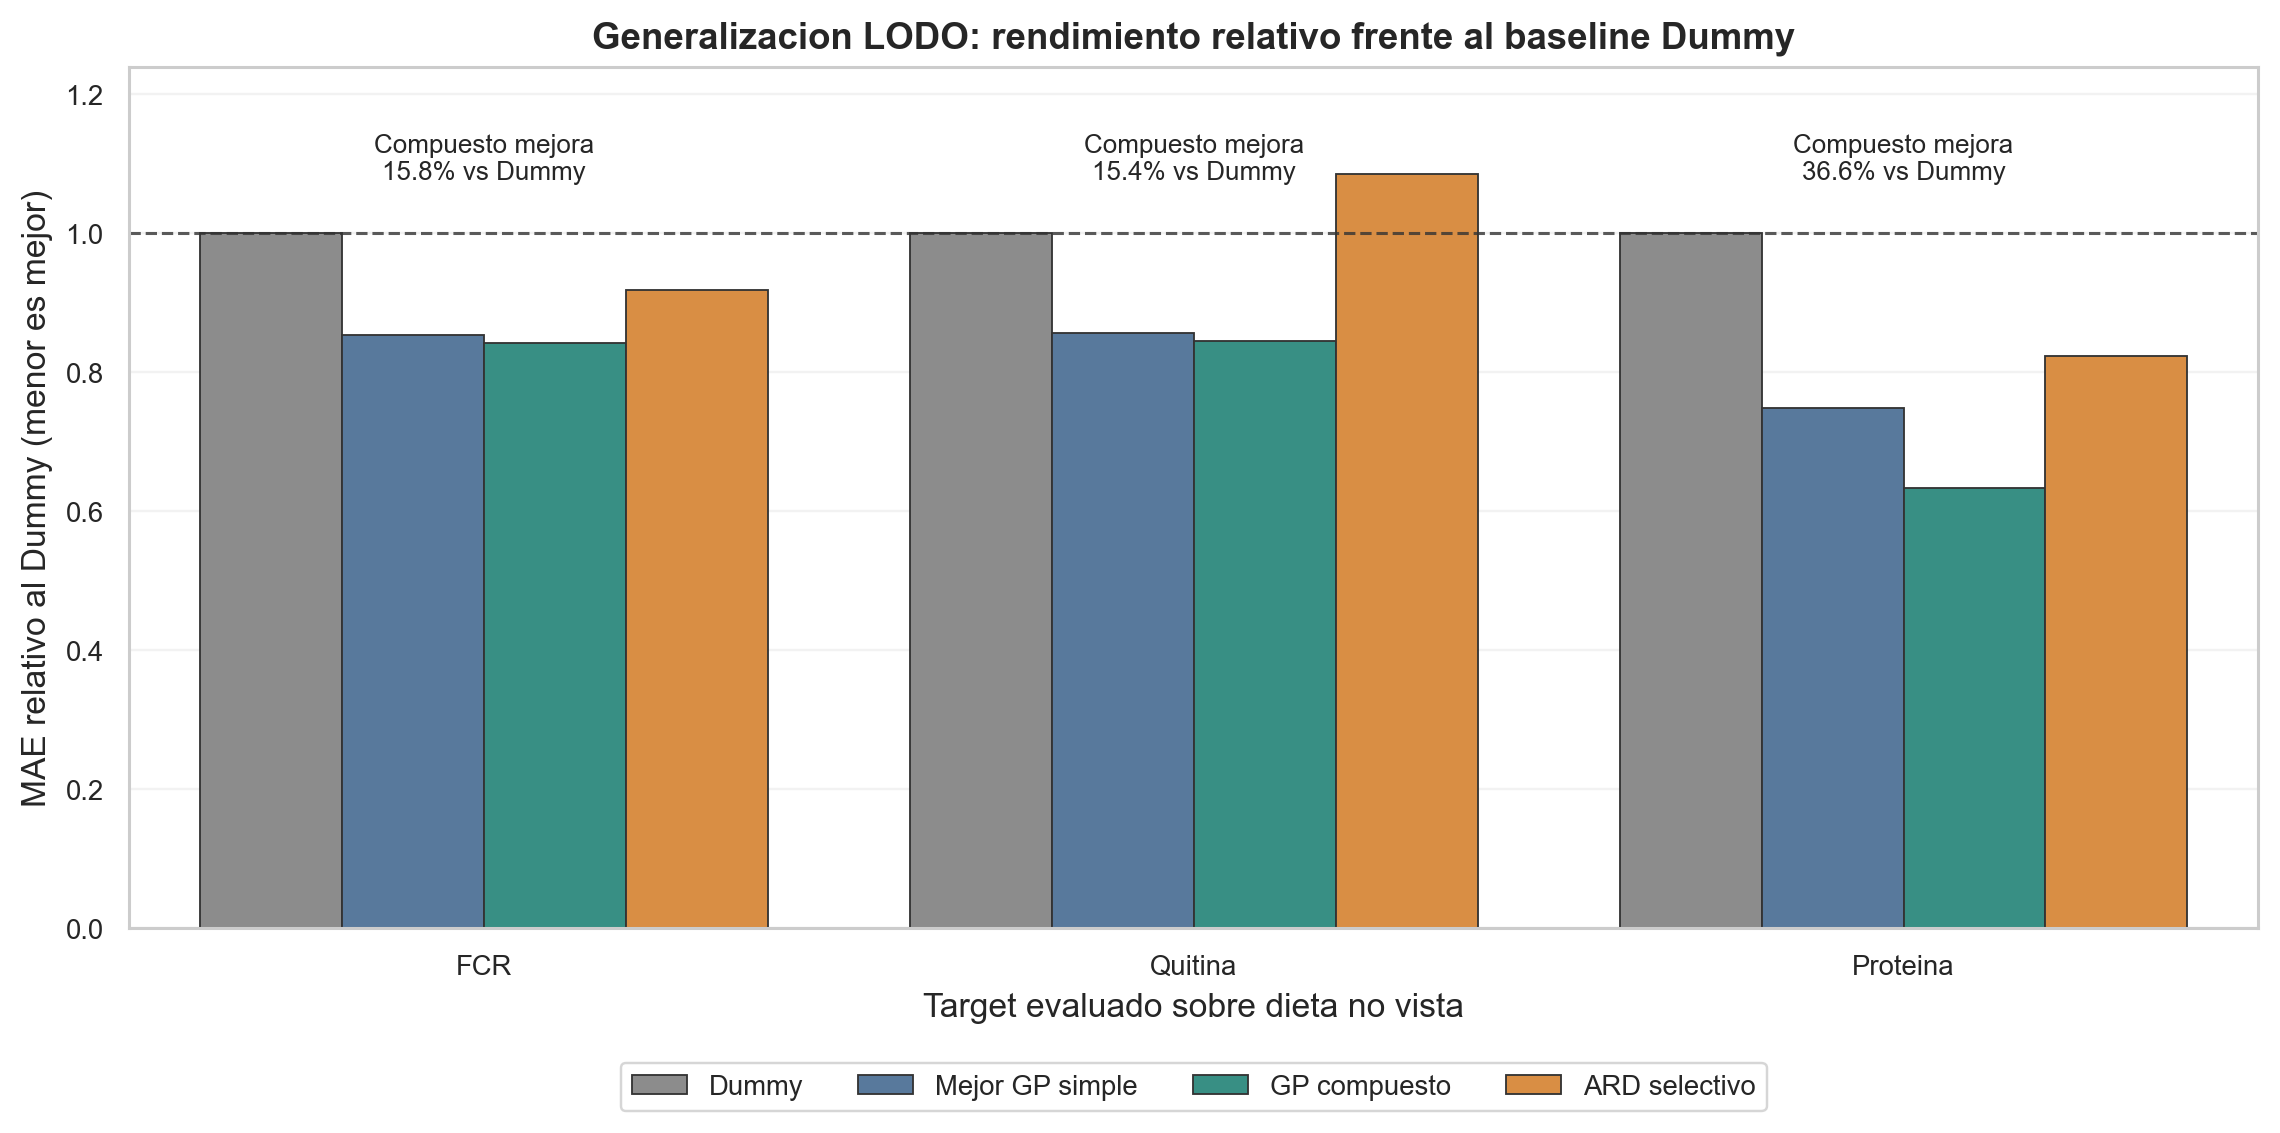
\includegraphics[width=0.95\textwidth]{assets/fig_01_lodo_generalization_vs_dummy.png}
    \caption{Rendimiento relativo de los modelos frente al baseline Dummy en validación LODO. Valores inferiores a \(1\) indican menor MAE que Dummy y, por tanto, mejor capacidad predictiva sobre dietas no vistas.}
    \label{fig:lodo_generalization_vs_dummy}
\end{figure}
\FloatBarrier

No obstante, esta mejora agregada no debe interpretarse como una generalización uniforme. La Figura~\ref{fig:error_by_left_out_diet} descompone el error por dieta retenida y muestra que la dificultad del problema depende de la formulación evaluada. En FCR, los errores son relativamente contenidos en varias dietas, aunque aparecen dietas más difíciles, como \texttt{Hoja50} y algunas formulaciones con orujo o quinoa. En quitina, la dificultad se concentra especialmente en dietas como \texttt{Orujo70}, \texttt{Orujo90} y \texttt{Control}, mientras que en proteína destacan errores elevados en dietas como \texttt{Orujo50} y algunas formulaciones con hoja.

\begin{figure}[htbp]
    \centering
    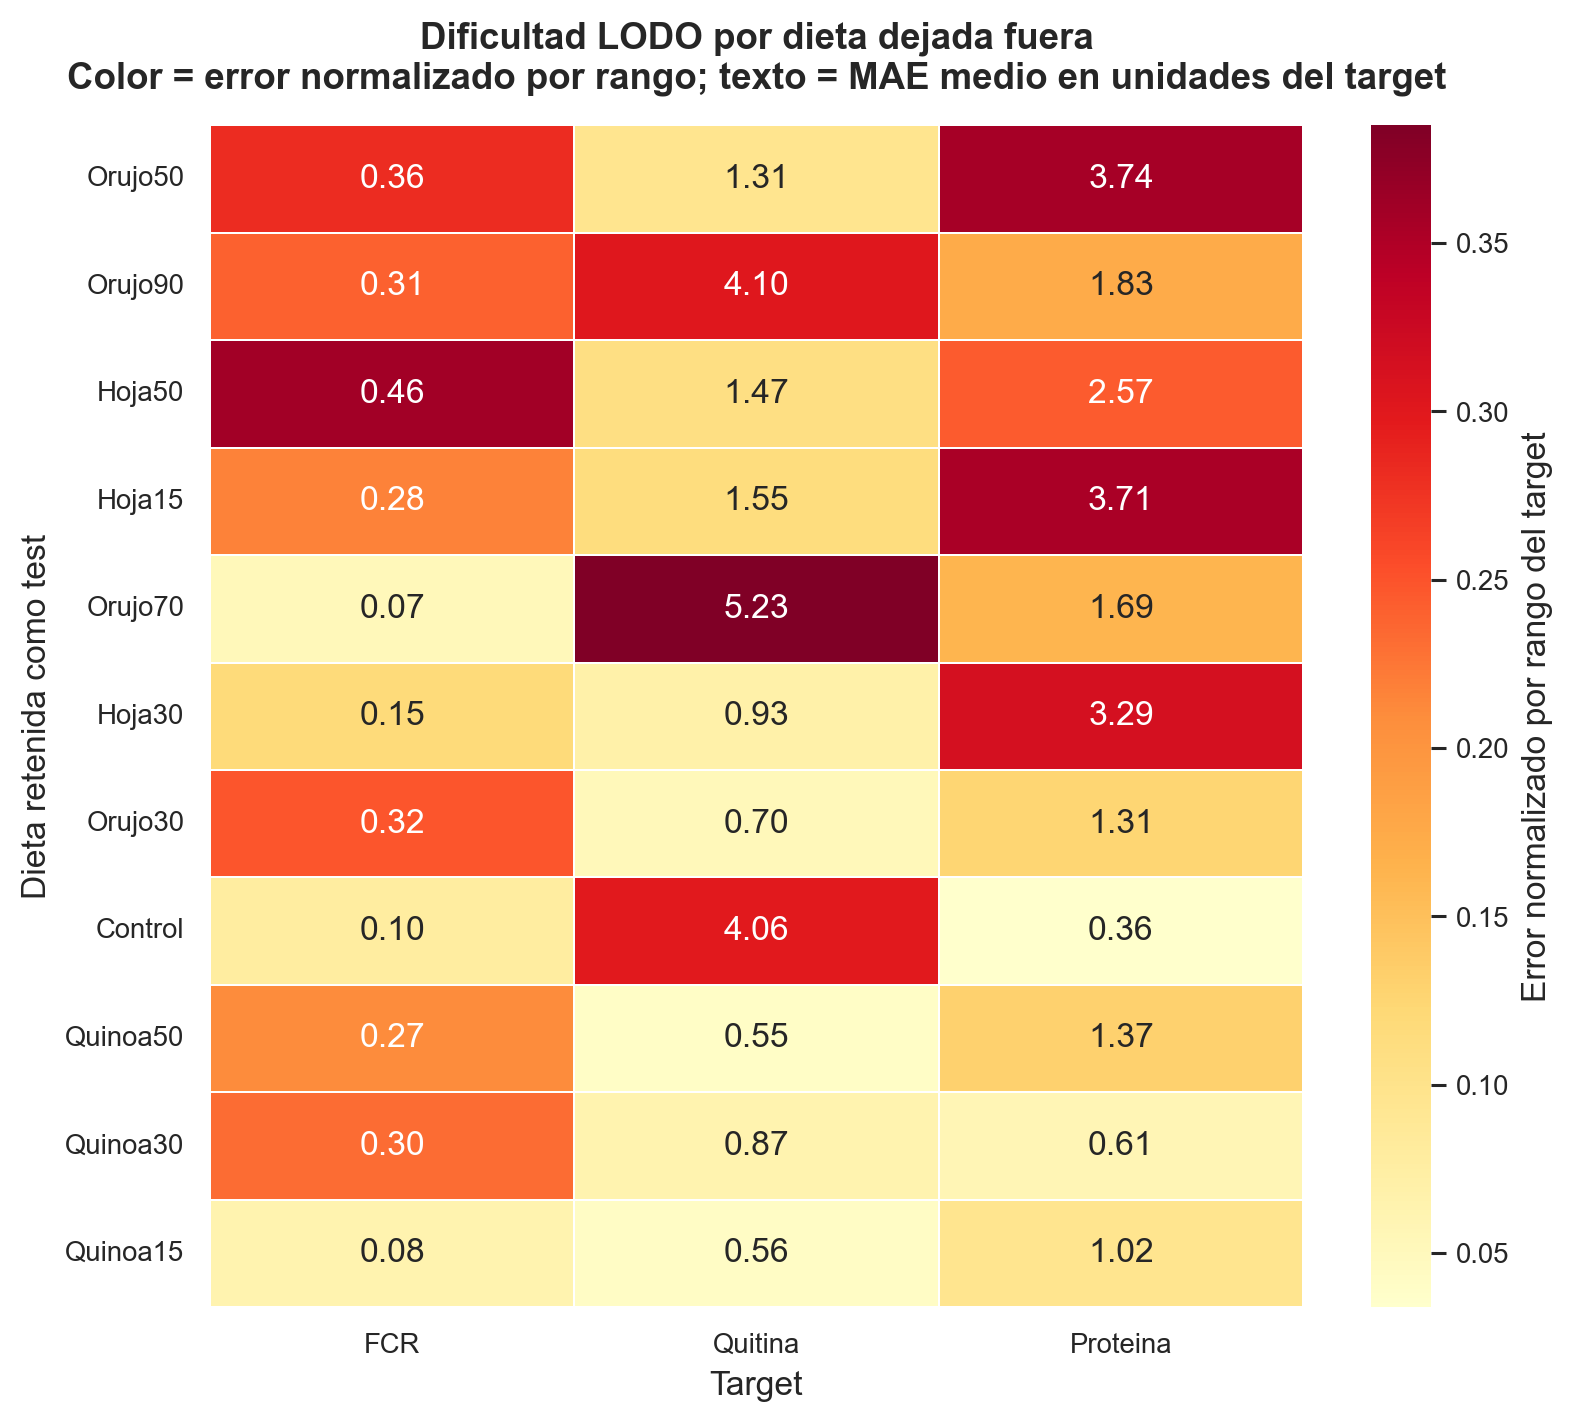
\includegraphics[width=0.72\textwidth]{assets/fig_02_error_by_left_out_diet.png}
    \caption{Dificultad de generalización por dieta retenida en el protocolo LODO. El color representa el error normalizado por el rango del objetivo y el texto muestra el MAE medio en las unidades originales de cada variable.}
    \label{fig:error_by_left_out_diet}
\end{figure}
\FloatBarrier

La lectura conjunta de ambas figuras es importante. La mejora frente al Dummy muestra que existe una señal aprendible en las variables nutricionales y de formulación, pero el mapa de errores evidencia que dicha señal no se transfiere igual a todas las dietas. Esto es coherente con la naturaleza del caso real: las respuestas de las larvas no dependen únicamente de una tendencia global asociada al porcentaje de inclusión o a la composición media, sino también de efectos específicos del subproducto, variabilidad experimental y posibles interacciones no completamente representadas en las variables disponibles.

En consecuencia, el resultado no permite afirmar que el GP resuelva por completo el problema de predicción de nuevas dietas. Sí permite, en cambio, defender que el modelo compuesto captura regularidades útiles más allá de la memorización de réplicas. La validación LODO actúa aquí como una prueba de generalización estructural: si el modelo mejora al Dummy aun cuando se retira una dieta completa, entonces parte de la información aprendida procede de relaciones compartidas entre dietas, y no solo de la repetición de observaciones muy similares dentro de una misma formulación.

\subsubsection{Expresividad geométrica del GP compuesto}
\label{subsubsec:expresividad_gp_compuesto}

Una vez comprobado que el GP aporta capacidad predictiva frente al baseline, la siguiente cuestión es qué tipo de estructura de covarianza resulta más adecuada para este caso real. Como se explicó en la Sección~\ref{subsec:gp_kernel}, el kernel no es únicamente un componente técnico del GP, sino el elemento que define las hipótesis a priori sobre la forma de la función que se desea aproximar. En este caso, la respuesta biológica de las larvas puede contener una tendencia global asociada a la composición nutricional de la dieta, pero también desviaciones locales debidas al tipo de subproducto, al porcentaje de inclusión y a la variabilidad experimental.

La Figura~\ref{fig:kernel_family_mae} compara distintas familias de kernel utilizando el MAE macro en el protocolo LODO. La comparación muestra que el kernel compuesto es el modelo más competitivo en los tres objetivos considerados. Esta diferencia es especialmente clara en proteína, donde el GP compuesto reduce de forma apreciable el error frente al Dummy y frente a los kernels simples. En quitina también se observa una mejora consistente respecto a las alternativas individuales, mientras que en FCR las diferencias entre varios kernels no lineales son más reducidas, aunque el compuesto se mantiene entre las mejores opciones.

\begin{figure}[htbp]
    \centering
    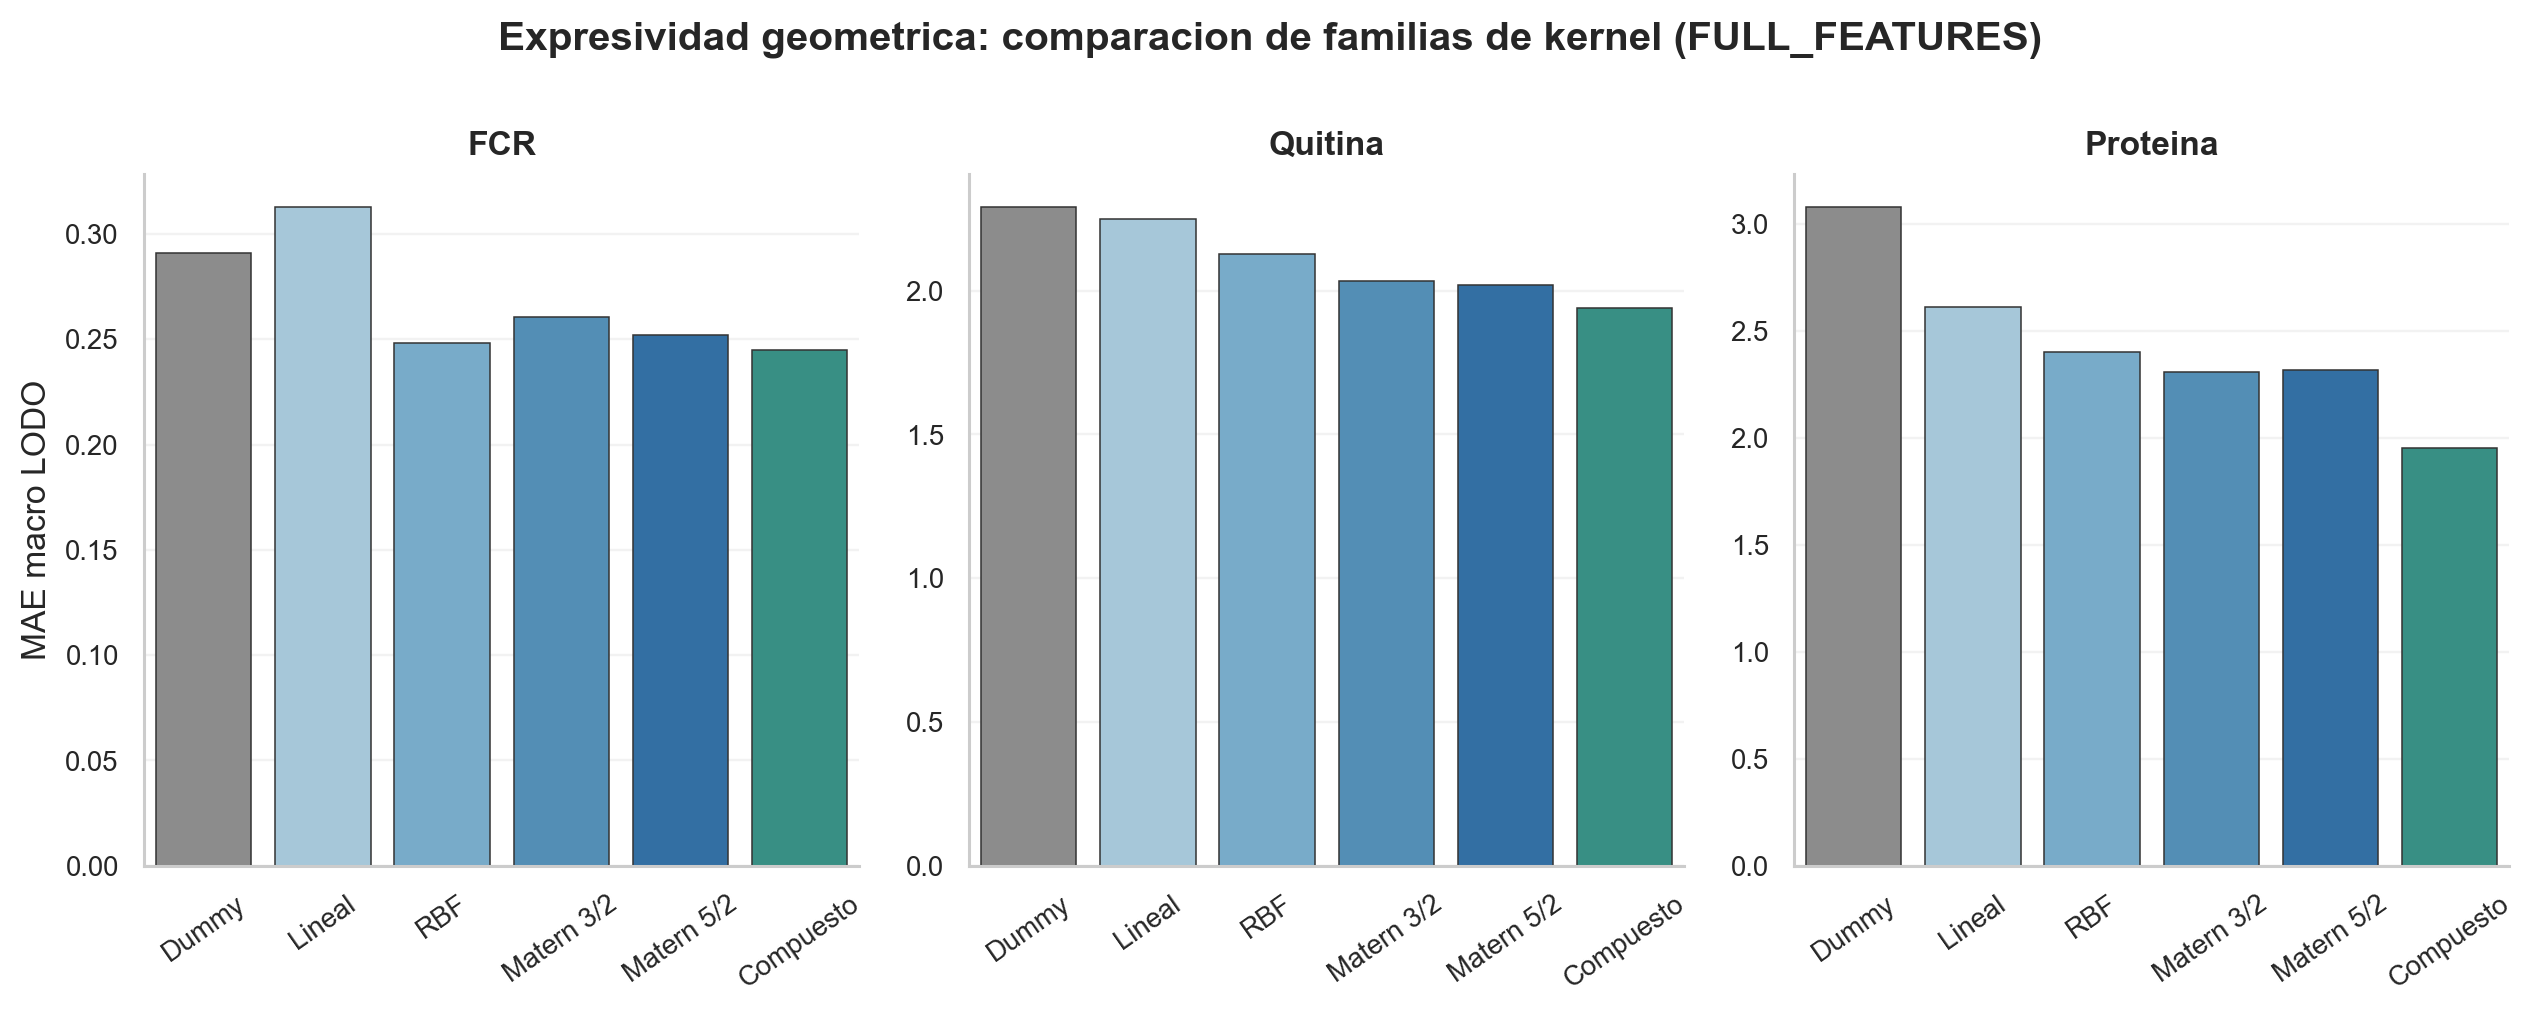
\includegraphics[width=0.95\textwidth]{assets/fig_04_kernel_family_mae.png}
    \caption{Comparación de familias de kernel en el caso real de \textit{Hermetia}. El eje vertical muestra el MAE macro obtenido mediante validación LODO; valores menores indican mejor generalización a dietas no vistas.}
    \label{fig:kernel_family_mae}
\end{figure}
\FloatBarrier

El kernel compuesto utilizado puede escribirse de forma esquemática como
\[
k(\bm{x},\bm{x}')
=
C_1\,k_{\text{Lineal}}(\bm{x},\bm{x}')
+
C_2\,k_{\text{Matérn }5/2}(\bm{x},\bm{x}')
+
k_{\text{White}}(\bm{x},\bm{x}').
\]
Esta suma permite combinar tres comportamientos complementarios. El término lineal recoge una tendencia global de la respuesta respecto a las variables de entrada, como el porcentaje de inclusión o la composición nutricional media. El término Matérn \(5/2\) introduce variaciones locales suaves, sin imponer la suavidad extrema del kernel RBF. Por último, el término de ruido blanco recoge variabilidad residual o experimental que no queda explicada por las covariables disponibles.

Esta estructura resulta razonable para el caso Entomotive porque las relaciones entre dieta y respuesta larvaria no tienen por qué ser puramente lineales. Por ejemplo, aumentar el porcentaje de un subproducto puede desplazar la respuesta en una dirección general, pero ese efecto puede variar según el tipo de subproducto y según el objetivo medido. Un kernel exclusivamente lineal puede ser demasiado rígido para capturar estas desviaciones, mientras que un kernel puramente local puede perder parte de la tendencia global común entre dietas. El kernel compuesto actúa como un compromiso: mantiene una componente interpretable de tendencia global y añade flexibilidad local para modelar desviaciones suaves alrededor de esa tendencia.

No obstante, este resultado debe interpretarse con prudencia. La superioridad del GP compuesto en la Figura~\ref{fig:kernel_family_mae} no significa que el modelo capture por completo la dinámica biológica del sistema, ni que pueda extrapolar con seguridad fuera del rango experimental observado. Lo que muestra es que, dentro del espacio cubierto por las dietas disponibles y bajo validación LODO, una estructura de covarianza que combina tendencia global, variación local y ruido experimental describe mejor los datos que las familias simples consideradas por separado.

Por tanto, el GP compuesto se adopta como modelo principal no porque elimine la incertidumbre del caso real, sino porque ofrece la mejor combinación observada entre flexibilidad y robustez. Esta lectura enlaza con el objetivo del TFG: construir un sustituto suficientemente informativo para analizar dietas no vistas y orientar futuras evaluaciones, sin presentar sus predicciones como una sustitución definitiva del ensayo experimental.

\subsubsection{Calibración práctica de la incertidumbre}
\label{subsubsec:calibracion_incertidumbre_caso_real}

Además de evaluar la precisión de la media predictiva, en este caso real interesa comprobar si la incertidumbre del GP aporta información útil sobre la fiabilidad de sus predicciones. Esta cuestión es especialmente relevante porque el objetivo no es únicamente interpolar dietas ya ensayadas, sino valorar si el modelo puede orientar decisiones sobre formulaciones no observadas. En este contexto, una predicción puntual con error puede seguir siendo útil si el modelo expresa una incertidumbre elevada en las regiones donde es probable que falle. Por el contrario, un modelo que comete errores grandes con intervalos demasiado estrechos resultaría poco fiable como herramienta prospectiva.

La Figura~\ref{fig:uncertainty_vs_error} compara, para cada objetivo, la desviación estándar predictiva del GP con el error absoluto cometido en las dietas retenidas por LODO. Esta representación permite analizar de forma práctica si las zonas donde el modelo declara mayor incertidumbre coinciden con aquellas donde el error real es mayor. La relación es más clara en quitina, donde se obtiene una correlación positiva entre incertidumbre y error. En este caso, el GP tiende a asignar mayor desviación estándar a observaciones que efectivamente resultan más difíciles de predecir, por lo que la incertidumbre actúa como una señal útil de cautela.

\begin{figure}[htbp]
    \centering
    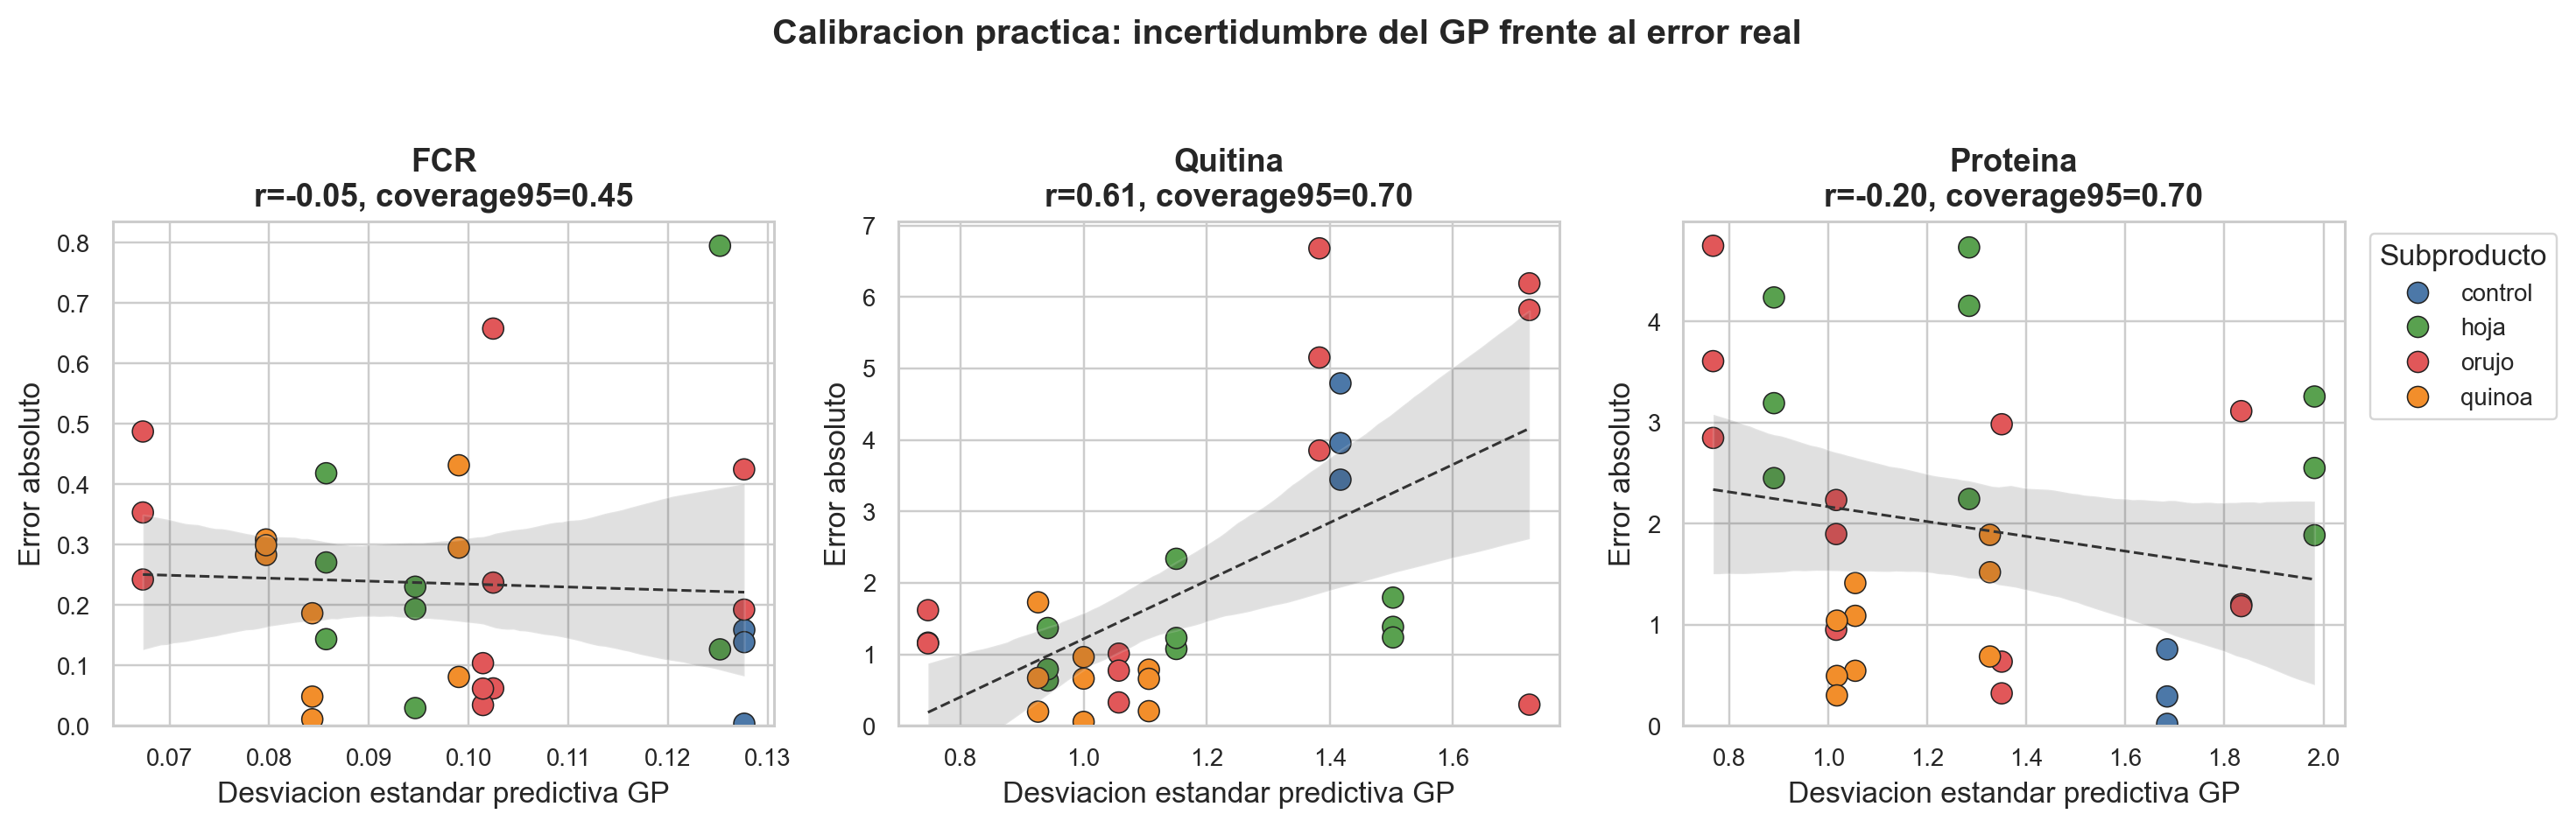
\includegraphics[width=0.95\textwidth]{assets/fig_05_uncertainty_vs_error.png}
    \caption{Relación entre la desviación estándar predictiva del GP y el error absoluto observado en validación LODO. Cada punto corresponde a una observación evaluada en una dieta retenida; el color indica el tipo de subproducto.}
    \label{fig:uncertainty_vs_error}
\end{figure}
\FloatBarrier

En FCR y proteína, sin embargo, la calibración es más débil. En FCR la relación entre desviación estándar y error es prácticamente nula, lo que indica que el modelo no ordena bien los casos fáciles y difíciles según su incertidumbre. En proteína la relación también es limitada, e incluso aparecen errores relevantes en zonas donde el modelo no siempre asigna una incertidumbre proporcionalmente alta. Por tanto, la incertidumbre del GP no debe interpretarse como una medida perfectamente calibrada en todos los objetivos.

La Figura~\ref{fig:prediction_intervals_by_diet} muestra esta misma idea desde una perspectiva más aplicada, representando para cada dieta la media predictiva LODO junto con intervalos aproximados del \(95\,\%\). En varios casos, los intervalos proporcionan una lectura razonable del rango plausible de valores, pero también aparecen fallos relevantes en dietas concretas. Esto confirma que la incertidumbre es informativa como herramienta de diagnóstico, aunque no suficiente para garantizar por sí sola la validez de una predicción individual.

\begin{figure}[htbp]
    \centering
    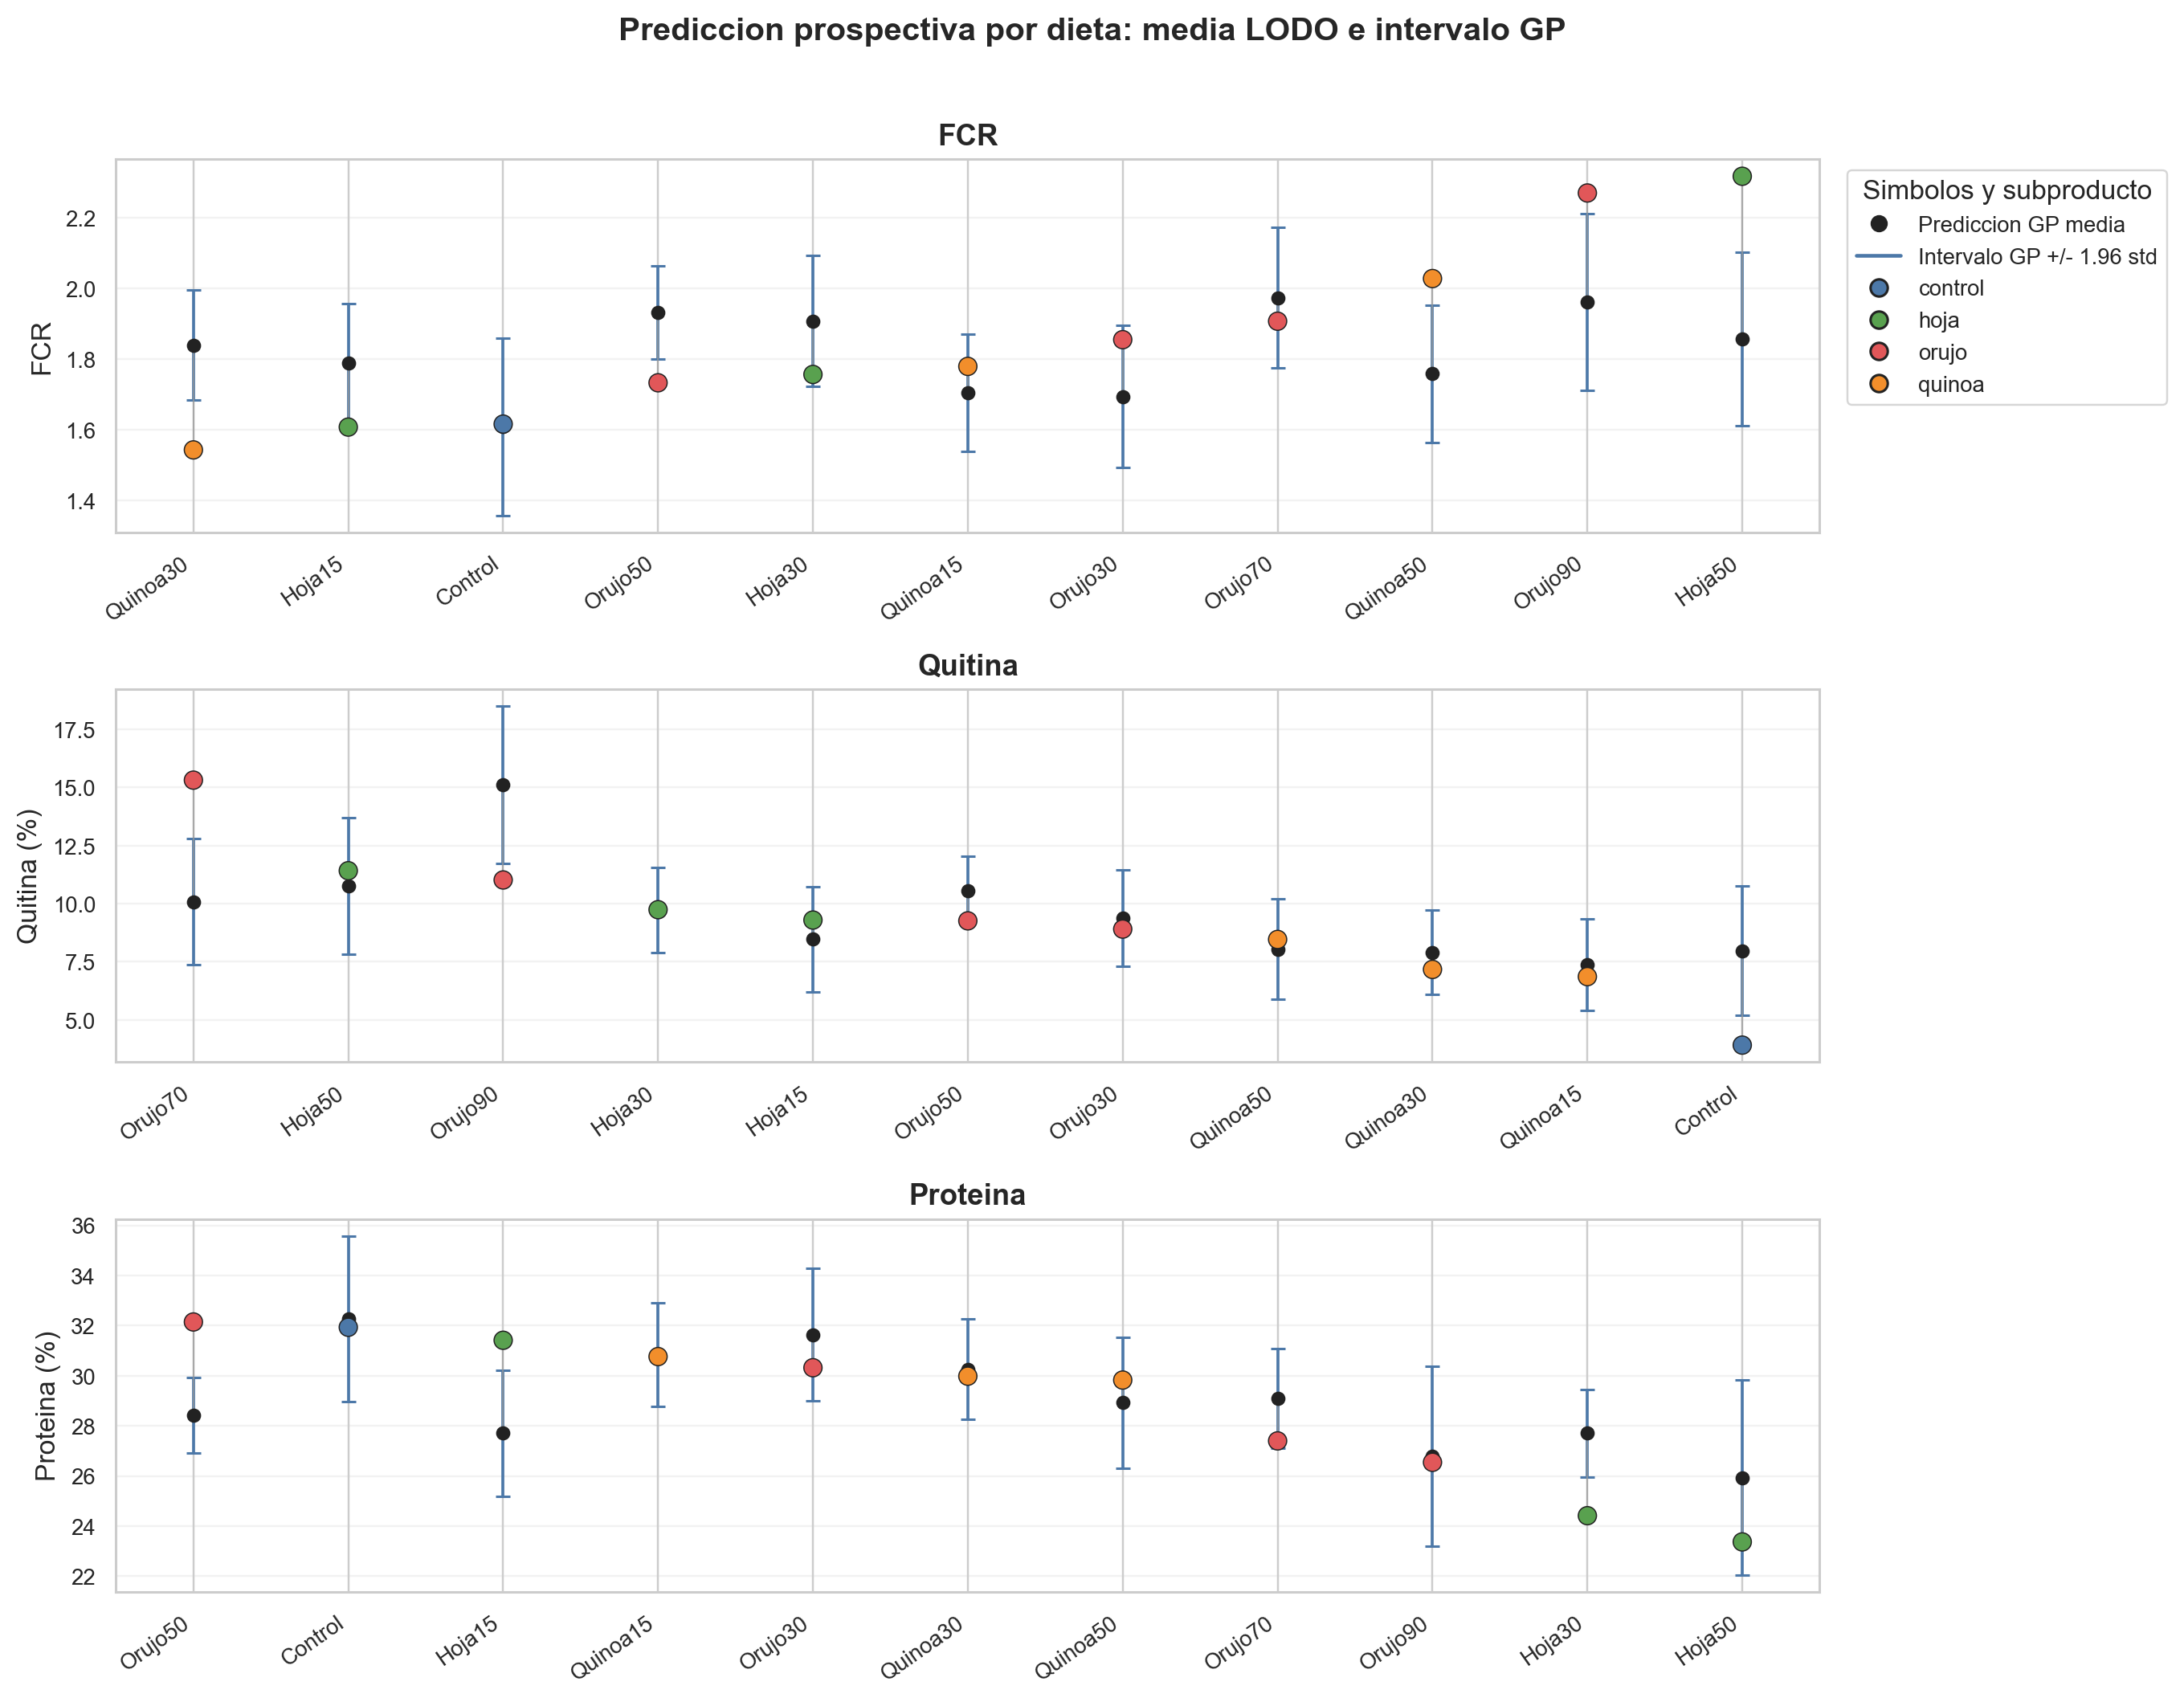
\includegraphics[width=0.95\textwidth]{assets/fig_06_prediction_intervals_by_diet.png}
    \caption{Predicción prospectiva por dieta bajo validación LODO. Los puntos negros representan la media predictiva del GP y las barras muestran intervalos aproximados del \(95\,\%\) construidos como \(\mu \pm 1.96\sigma\). Los puntos coloreados corresponden a los valores observados por tipo de subproducto.}
    \label{fig:prediction_intervals_by_diet}
\end{figure}
\FloatBarrier

La lectura conjunta de ambas figuras es que el GP aporta un valor diferencial respecto a modelos puramente puntuales, porque no solo devuelve una predicción media, sino también una estimación de incertidumbre. No obstante, esa incertidumbre está solo parcialmente calibrada. En quitina, la desviación estándar predictiva se relaciona mejor con el error real y permite identificar zonas de mayor riesgo. En FCR y proteína, la señal de incertidumbre es más débil.

En consecuencia, la incertidumbre del GP se interpreta en este trabajo como una señal de apoyo para la toma de decisiones, no como una garantía absoluta de fiabilidad. Su papel es especialmente útil para priorizar ensayos futuros y detectar regiones donde el modelo reconoce mayor desconocimiento. Sin embargo, cualquier candidato propuesto a partir del sustituto debe entenderse como una hipótesis experimental pendiente de validación, no como una conclusión cerrada sobre el rendimiento real de una nueva dieta.

\subsubsection{Viabilidad prospectiva y propuesta de pre-\emph{infill}}
\label{subsubsec:preinfill_caso_real}

El último paso del análisis consiste en estudiar si el modelo sustituto es suficientemente informativo como para orientar una posible fase futura de experimentación. A diferencia del experimento de benchmarks, en el caso real no se ejecuta todavía un ciclo físico de \emph{infill}: no se ensayan nuevas dietas ni se actualiza el dataset con observaciones adicionales. Lo que se plantea es una fase previa, o pre-\emph{infill}, en la que el GP entrenado se utiliza para recorrer un espacio factible de formulaciones y priorizar candidatos que podrían ser evaluados posteriormente.

Para ello se emplea el criterio de Expected Improvement introducido en la Sección~\ref{sec:muestreo_inicial} y formulado en la Ecuación~\eqref{eq:ei}, adaptando la orientación de cada objetivo. En FCR se busca minimizar el valor observado, mientras que en quitina y proteína se busca maximizarlo. El espacio de búsqueda prospectivo se define a partir de los subproductos considerados en el caso real, esto es, hoja, orujo y quinoa, y de porcentajes de inclusión dentro del rango observado. Sobre este dominio se construye una rejilla densa con incrementos del \(1\,\%\), excluyendo las formulaciones ya ensayadas para que el candidato propuesto corresponda a un punto nuevo.

La Tabla~\ref{tab:incumbents_candidatos_ei} resume la diferencia entre el mejor punto ya observado y el candidato priorizado por EI. El \emph{incumbent} observado corresponde a la mejor dieta medida experimentalmente para cada objetivo individual. En cambio, el candidato EI no es una dieta validada, sino una formulación no ensayada que el modelo considera informativa bajo el equilibrio entre explotación e incertidumbre.

\begin{table}[htbp]
    \centering
    \small
    \caption{Incumbents observados y candidatos prospectivos priorizados por EI.}
    \label{tab:incumbents_candidatos_ei}
    \renewcommand{\arraystretch}{1.15}
    \setlength{\tabcolsep}{4pt}
    \begin{tabularx}{\textwidth}{@{}p{1.5cm} p{3cm} p{2.6cm} p{2.6cm} p{1.1cm} X@{}}
        \toprule
        \textbf{Objetivo} 
        & \textbf{Incumbent observado} 
        & \textbf{Candidato EI} 
        & \textbf{Predicción del candidato} 
        & \textbf{EI} 
        & \textbf{Lectura} \\
        \midrule

        FCR
        & \texttt{Quinoa30}: \(1.543\)
        & \texttt{Quinoa16}
        & \(1.726 \pm 0.065\)
        & \(2.7{\cdot}10^{-5}\)
        & La media predicha no mejora al incumbent, por lo que el candidato debe interpretarse como exploratorio. \\

        Quitina
        & \texttt{Orujo70}: \(15.318\,\%\)
        & \texttt{Orujo89}
        & \(12.658 \pm 1.061\,\%\)
        & \(0.002\)
        & La propuesta se sitúa en una región de orujo con alta inclusión, pero no supera en media al mejor valor observado. \\

        Proteína
        & \texttt{Orujo50}: \(32.147\,\%\)
        & \texttt{Orujo31}
        & \(30.938 \pm 0.912\,\%\)
        & \(0.038\)
        & EI prioriza un punto nuevo de orujo, aunque la media predicha sigue por debajo del incumbent observado. \\

        \bottomrule
    \end{tabularx}
\end{table}
\FloatBarrier

La Tabla~\ref{tab:incumbents_candidatos_ei} permite distinguir de forma explícita entre el mejor resultado ya medido y el punto nuevo sugerido por EI. En los tres objetivos, el candidato EI aparece separado del incumbent observado. Esta separación es importante porque evita confundir dos conceptos distintos: el incumbent es una evidencia experimental ya medida, mientras que el candidato EI es una hipótesis propuesta por el modelo para una posible evaluación futura. Además, las medias predichas de los candidatos no superan claramente a los incumbents observados; por tanto, su selección está asociada principalmente al valor exploratorio de EI y a la incertidumbre del GP, no a una mejora media ya demostrada.

Esta distinción es especialmente relevante en un caso real con pocos datos. Por ejemplo, para FCR el incumbent observado sigue siendo \texttt{Quinoa30}; para quitina, \texttt{Orujo70}; y para proteína, \texttt{Orujo50}. Los candidatos EI no sustituyen a estos resultados experimentales. Su papel es diferente: señalan dónde podría merecer la pena invertir un nuevo ensayo si se quisiera continuar el estudio. En otras palabras, el GP no cierra la decisión experimental, sino que reduce el espacio de búsqueda y ayuda a seleccionar formulaciones con mayor valor informativo.

\begin{figure}[htbp]
    \centering
    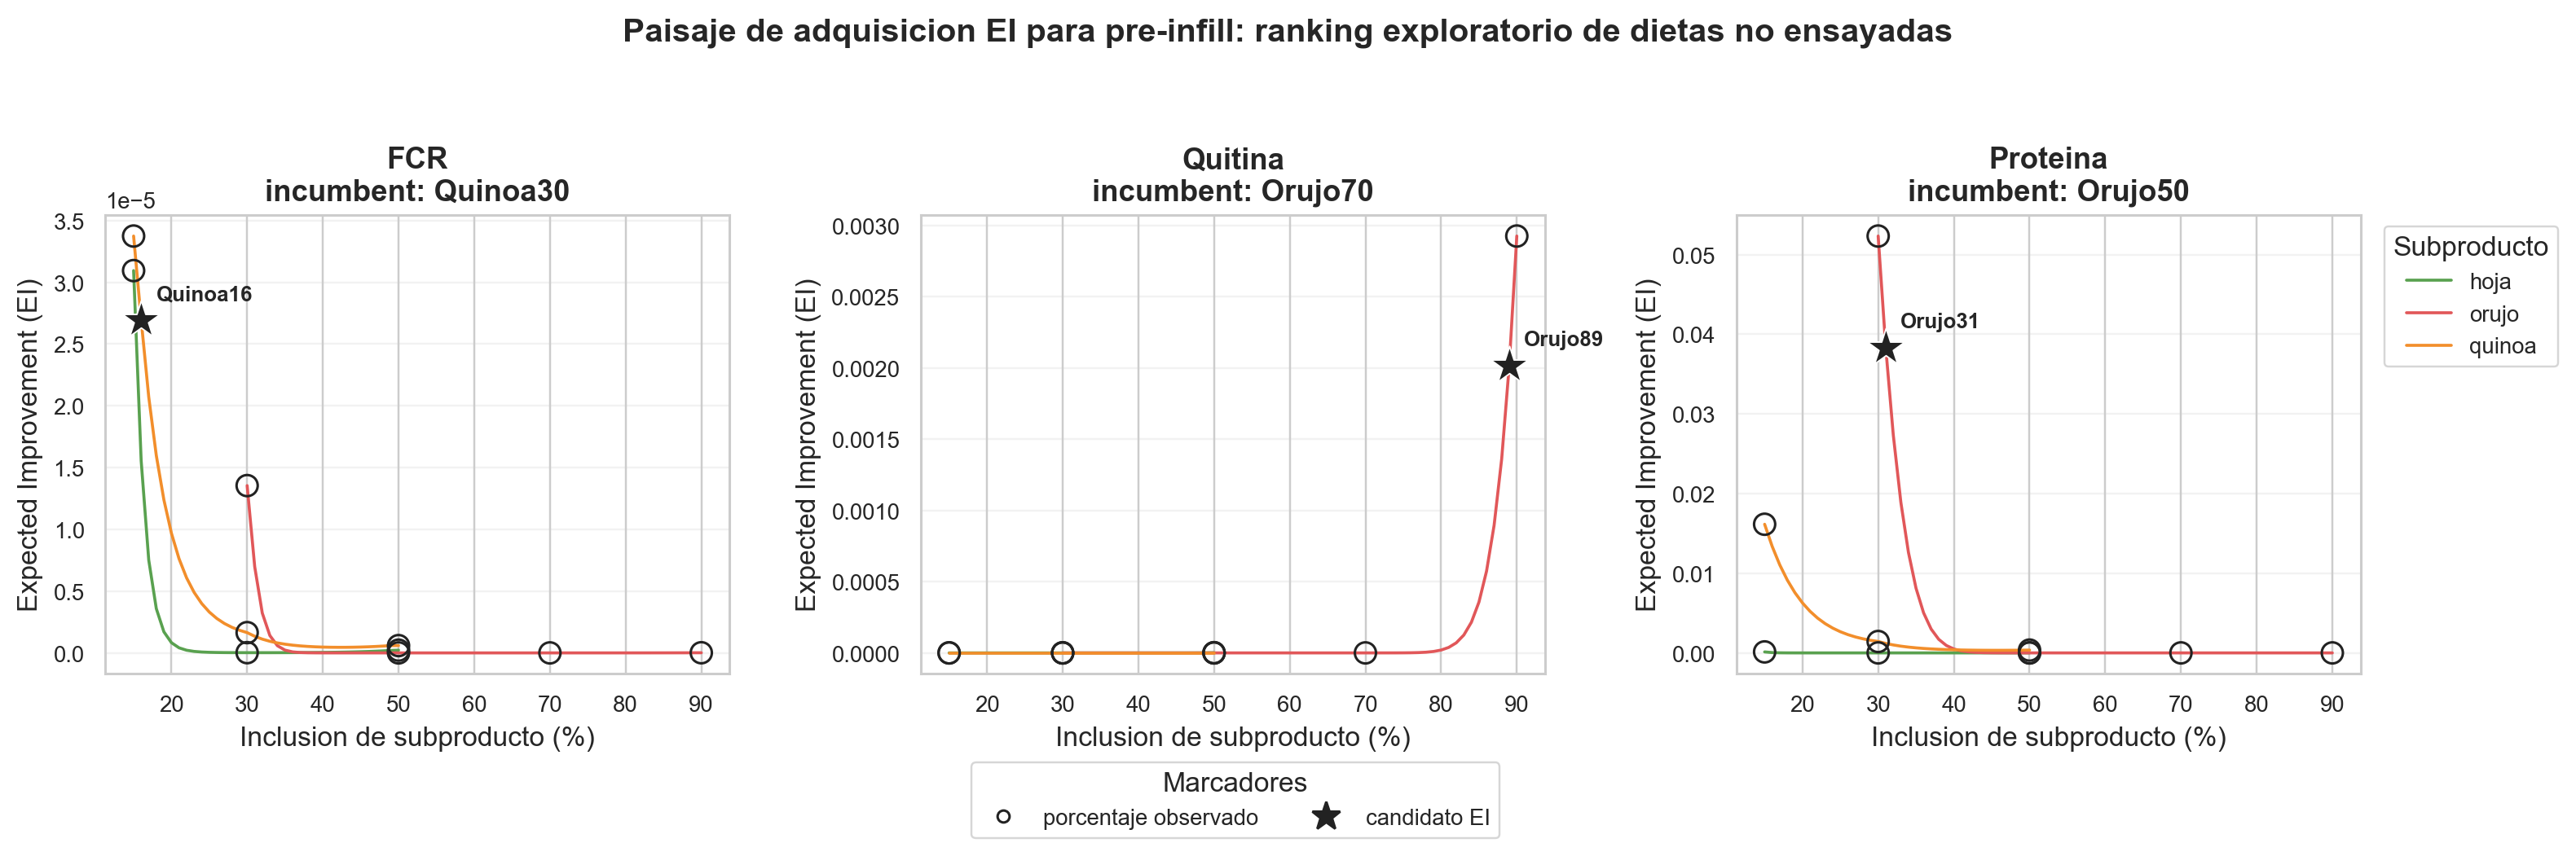
\includegraphics[width=0.95\textwidth]{assets/fig_08_ei_candidate_landscape.png}
    \caption{Paisaje prospectivo de EI sobre la rejilla factible de formulaciones. Los máximos de EI identifican puntos candidatos para una posible evaluación futura, combinando predicción media e incertidumbre del GP.}
    \label{fig:ei_candidate_landscape}
\end{figure}
\FloatBarrier

En conjunto, el pre-\emph{infill} muestra que el modelo sustituto es utilizable como herramienta de cribado prospectivo. La validación LODO indica que el GP compuesto aprende una señal predictiva útil; el análisis de incertidumbre muestra que esa señal debe manejarse con cautela; y EI permite transformar ambas piezas de información en propuestas concretas de ensayo. Por tanto, la conclusión no es que \texttt{Quinoa16}, \texttt{Orujo89} u \texttt{Orujo31} sean nuevas dietas óptimas demostradas, sino que constituyen candidatos razonables para una siguiente iteración experimental.
